\documentclass[a4paper,12pt]{article} % Define o tipo de documento e suas configurações básicas
\usepackage[utf8]{inputenc} % Permite o uso de caracteres especiais no texto
\usepackage{indentfirst} % Adiciona indentação no primeiro parágrafo de cada seção
\usepackage[T1]{fontenc} % Especifica a codificação de fonte a ser usada
\usepackage{geometry} % Permite a configuração das margens do documento
\geometry{a4paper, margin=2cm} % Define o tamanho e as margens do papel
\usepackage{amsmath} % Pacote para equações matemáticas
\usepackage[brazil,english]{babel} % Define o idioma principal e secundário do documento
\usepackage{graphicx} % Pacote para inclusão de gráficos
\usepackage{hyperref} % Pacote para adicionar hiperlinks
\usepackage{float} % Melhora o posicionamento de elementos flutuantes
\usepackage{multirow} % Permite a criação de células em tabelas ocupando múltiplas linhas
\usepackage{csquotes} % Pacote para citações
\usepackage{minted} % Pacote para inclusão de código fonte
\usepackage{xcolor} % Pacote para definição de cores
\definecolor{bg}{rgb}{0.95,0.95,0.95} % Define uma cor de fundo para o ambiente de código
\usemintedstyle{default} % Define o estilo de formatação do código
\usepackage[nottoc]{tocbibind} % Includes "References" in the table of contents
\usepackage{fvextra}
\usepackage{csquotes}
\title{Modelos de Aprendizado de Máquina aplicados à Previsão do Status de Empréstimo}
\author{Breno Cauã Rodrigues da Silva}
\date{}

\begin{document}
\maketitle

\selectlanguage{brazil}
\begin{abstract}
Este relatório descreve uma análise comparativa entre modelos de classificação aplicados à previsão do status de empréstimo. O conjunto de dados utilizado foi obtido do Kaggle e contém informações sobre solicitantes de empréstimo com base no imóvel, sendo um empréstimo imobiliário. O objetivo é construir um modelo de aprendizado de máquina para prever se o empréstimo será aprovado ou rejeitado. Diversos modelos foram treinados e avaliados quanto à sua acurácia. Os resultados indicam que o modelo de Árvore de Decisão obteve as melhores métricas, sendo uma delas, acurácia, com 92,21\%. Este relatório detalha os processos e etapas para obter o melhor classificador, desde os códigos utilizados até a análises e explicações ao decorrer do relatório, bem como as etapas de pré-processamento, análise exploratória, treinamento e teste e avaliação de modelos.
\end{abstract}

\selectlanguage{english}
\begin{abstract}
This report describes a comparative analysis between classification models applied to loan status prediction. The dataset used was obtained from Kaggle and contains information about loan applicants based on the property, being a real estate loan. The goal is to build a machine learning model to predict whether the loan will be approved or rejected. Several models were trained and evaluated for their accuracy. The results indicate that the Decision Tree model obtained the best metrics, one of them being accuracy, with 92.21\%. This report details the processes and steps to obtain the best classifier, from the codes used to the analyzes and explanations throughout the report, as well as the pre-processing, exploratory analysis, training and testing and model evaluation steps.
\end{abstract}

\selectlanguage{brazil}
\newpage


\section{Introdução}
A aprovação de empréstimos é um ponto crucial em operações financeiras, mas envolve riscos consideráveis para os bancos e instituições financeiras. Um dos principais focos do setor bancário é aprimorar a avaliação de solicitações de crédito, uma vez que o risco de crédito surge quando os clientes não cumprem suas obrigações financeiras com o banco \cite{maciel2015analise}. A capacidade de prever com precisão se um solicitante terá seu empréstimo aprovado ou não é fundamental para minimizar perdas e maximizar lucros, especialmente em um cenário econômico dinâmico e competitivo.

Nesse contexto, a aplicação de técnicas avançadas de análise de dados se torna cada vez mais relevante. Uma das características que têm sido objeto de discussão em Ciência de Dados está relacionada com o volume de dados, especialmente ao se tratar do que chamamos de megadados (Big Data) \cite{morettin2021estatistica}, com a ascensão do Big Data, as instituições financeiras têm acesso a uma quantidade massiva de informações sobre os solicitantes de empréstimos, incluindo histórico de crédito, informações pessoais, dados de emprego e muito mais. Utilizando esses dados de forma eficaz, é possível desenvolver modelos preditivos robustos que podem auxiliar na tomada de decisões relacionadas à concessão de empréstimos.

Aprendizado de Máquina (Machine Learning) é uma área da Inteligência Artificial (IA) que visa o desenvolvimento de técnicas computacionais para o aprendizado, bem como a construção de sistemas capazes de adquirir conhecimento de tal forma que esse processo seja automático \cite{monard2003conceitos}. As aplicações do Aprendizado de Máquina eram, originalmente, de cunho estritamente computacional. No entanto, desde o final dos anos 90, essa área expandiu seus horizontes e as aplicações de Aprendizado de Máquina começaram a ter muitas intersecções com as de Estatística \cite{izbicki2020aprendizado}. Essa interseção resultou em uma área híbrida chamada Aprendizado Estatístico de Máquina, que combina técnicas de ambas as áreas para criar algoritmos mais poderosos e flexíveis (veja \cite{morettin2021estatistica}, lá são explorados esses termos e essas técnicas). Os algoritmos de Aprendizado de Máquina podem aprender com os dados históricos e identificar padrões complexos que podem não ser facilmente perceptíveis aos analistas humanos. Isso permite a construção de modelos de classificação capazes de prever com precisão o resultado de uma solicitação de empréstimo com base em uma série de variáveis e características do solicitante.

Este relatório visa fornecer uma abrangente visão do problema de previsão de aprovação de empréstimos, abordando desde a metodologia utilizada até os resultados alcançados durante o estudo. Ao longo do documento, serão discutidos os processos de pré-processamento de dados, análise exploratória, seleção e treinamento de modelos, bem como a avaliação do desempenho dos mesmos. Espera-se que as informações e \textit{insights} apresentados possam contribuir significativamente para o aprimoramento das práticas de concessão de empréstimos e para a redução dos riscos associados a essas operações financeiras.

\section{Materiais e Métodos}
\subsection{Conjunto de Dados}
O conjunto de dados utilizado neste estudo foi obtido do \href{https://www.kaggle.com/datasets/bhavikjikadara/loan-status-prediction/data}{\textbf{Kaggle}}, uma plataforma de Ciência de Dados que oferece uma ampla variedade de conjuntos de dados e exemplos em diferentes linguagens de programação. Este conjunto de dados contém informações sobre solicitações de empréstimo com base em propriedades imobiliárias. Consiste em 381 linhas e 13 colunas, apresentando os seguintes atributos:

\begin{itemize}
    \item \textbf{Loan ID:} Identificação única do empréstimo;
    \item \textbf{Gender:} Gênero do requerente (masculino ou feminino);
    \item \textbf{Married:} Estado civil do requerente (casado ou não casado);
    \item \textbf{Dependents:} Número de dependentes do requerente;
    \item \textbf{Education:} Nível de educação do requerente (graduado ou não graduado);
    \item \textbf{Self Employed:} Se o requerente é autônomo (Sim/Não);
    \item \textbf{ApplicantIncome:} Renda do requerente;
    \item \textbf{CoapplicantIncome:} Renda do co-requerente (outra pessoa que contribui para o pagamento do empréstimo);
    \item \textbf{Loan Amount:} Valor do empréstimo solicitado em milhares;
    \item \textbf{Loan Amount Term:} Prazo do empréstimo em meses;
    \item \textbf{Credit History:} Histórico de crédito atendendo às diretrizes (0/1);
    \item \textbf{Property Area:} Área de localização da propriedade do requerente (urbana, semiurbana ou rural);
    \item \textbf{Loan Status:} Status do empréstimo (aprovado ou não aprovado), que é a variável alvo que se pretende prever. Pode ter dois valores: 0 (não aprovado) ou 1 (aprovado).
\end{itemize}

Esses atributos fornecem informações essenciais sobre os candidatos a empréstimos, bem como detalhes dos empréstimos solicitados. São fundamentais para compreender e modelar o processo de aprovação de empréstimos.

\subsection{Metodologia}
O processo de análise e modelagem dos dados para predição, seguiu as seguintes etapas:

\begin{enumerate}
    \item \textbf{Pré-processamento de Dados:} Esta etapa envolveu a limpeza e preparação dos dados brutos para análise. Isso incluiu tratamento de valores ausentes, codificação de variáveis categóricas, normalização ou padronização de dados numéricos e outras transformações necessárias para garantir a qualidade e consistência dos dados;
    \item \textbf{Análise Exploratória de Dados (AED):} Nesta fase, foram realizadas análises estatísticas e visualizações gráficas para entender a distribuição dos dados, identificar padrões, relações e tendências nos dados. Isso permitiu uma compreensão mais profunda do conjunto de dados e se torna decisivo caso seja necessário realizar \textit{redução de dimensionalidade};
    \item \textbf{Separação  do Conjunto de Dados em Treino e Teste:} Esta etapa é onde o conjunto de dados é dividido em duas partes distintas: uma para treinamento do modelo e outra para teste da sua eficácia. Essa abordagem é fundamental para avaliar o desempenho do modelo em dados não vistos durante o treinamento, garantindo sua capacidade de generalização para situações reais;
    \item \textbf{Desenvolvimento e Treinamento de Modelos:} Diversos algoritmos de classificação foram explorados e treinados utilizando o conjunto de dados reservado para treino. Foram considerados modelos como Árvores de Decisão, Florestas Aleatórias, Regressão Logística, Redes Neurais, entre outros. Cada modelo foi ajustado utilizando validação (conjunto de teste) e otimização de hiperparâmetros para garantir o melhor desempenho possível;
    \item \textbf{Avaliação do Desempenho dos Modelos:} Os modelos treinados foram avaliados utilizando métricas de desempenho adequadas para problemas de classificação, como Acurácia, Matriz de Confusão e Curva ROC. Essas métricas forneceram compreensão sobre a capacidade de generalização e precisão de cada modelo em prever o status de aprovação de empréstimos.
\end{enumerate}

Para conduzir as análises e estimativas neste estudo, foi adotada a linguagem de programação Python, utilizando a IDE \href{https://colab.research.google.com/}{\textit{\textbf{Google Colaboratory}}} na versão 3.10.12. Foram empregadas as seguintes bibliotecas para implementação das diversas etapas do processo:

\begin{itemize}
    \item \textbf{NumPy:} Essa biblioteca é fundamental para realizar operações matemáticas, lógicas e estatísticas eficientes em arrays multidimensionais ou matrizes \cite{numpy}.
    \item \textbf{Pandas:} Utilizada para manipulação e análise de dados, o Pandas oferece estruturas de dados flexíveis e poderosas, permitindo o processamento de conjuntos de dados de forma intuitiva \cite{pandas, mckinney-proc-scipy-2010}.
    \item \textbf{Matplotlib:} Essa biblioteca é amplamente utilizada para criação de visualizações gráficas, incluindo gráficos de linha, histogramas, dispersão, barras, entre outros \cite{matplotlib}.
    \item \textbf{Seaborn:} Complementar ao Matplotlib, o Seaborn oferece uma interface de alto nível para criação de gráficos estatísticos atrativos e informativos. Ele é especialmente útil para visualização de dados complexos \cite{seaborn}.
    \item \textbf{Scikit-learn (Sklearn):} Essa biblioteca é uma ferramenta poderosa e eficiente para construção e avaliação de modelos de Machine Learning. Ela oferece uma ampla variedade de algoritmos de classificação, regressão, agrupamento, entre outros, bem como ferramentas para pré-processamento de dados e avaliação de modelos \cite{sklearn, sklearn_api}.
\end{itemize}

Veja o Código (1), que mostra a importação das bibliotecas que serão utilizadas para o estudo.
\begin{center}
\textbf{Código 01:} Importação dos dados. 
\begin{minted}[linenos, fontsize=\footnotesize, bgcolor=bg]{python}
# Importação e Pré-processamento
import numpy as np
import pandas as pd

# Análise Exploratória
import matplotlib.pyplot as plt
import seaborn as sns
sns.set(style='whitegrid')

# Separação do Conjunto de Dados
from sklearn.model_selection import train_test_split

# Classificação: Treinamento e Teste
from sklearn.tree import DecisionTreeClassifier # Árvore de Decisão
from sklearn.neighbors import KNeighborsClassifier # kNN
from sklearn.naive_bayes import GaussianNB # Naive Bayes
from sklearn.linear_model import LogisticRegression
from sklearn.neural_network import MLPClassifier # Redes Neurais
from sklearn.svm import SVC # SVM
from sklearn.ensemble import RandomForestClassifier, VotingClassifier # Assembly Methods

# Avaliação
from sklearn.metrics import accuracy_score, roc_curve, auc
from sklearn.metrics import confusion_matrix as cm

# Outras bibliotecas usadas
import warnings
warnings.filterwarnings('ignore')
from itertools import product
#import random
\end{minted}
\end{center}

É válido falar que as bibliotecas não comentadas anteriormente porém, presentes no Código (1) foram usadas em um único e específico momento. Por está  razão, não se foi falado delas antes porém, estão presentes nas referências. Veja \cite{python-warnings, python-itertools, python-random}.

\section{Resultados e Discussões}
\subsection{Importação e Pré-Processamento}
Sendo uma etapa de suma importância para encontrar o melhor classificador, temos a etapa de \textit{Importação e Pré-Processamento}, na qual são realizadas diversas manipulações e transformações nos dados. Isso inclui o tratamento de dados faltantes, normalização de variáveis, entre outros procedimentos. A seguir, apresenta-se o Código (2) utilizado para importar os dados.
\begin{center}
\textbf{Código 02:} Importação dos dados. 
\begin{minted}[linenos, fontsize=\footnotesize, bgcolor=bg]{python}
# Conectando ao Google Drive
from google.colab import drive
drive.mount('/content/drive')

# Importando o arquivo CSV
path = '/content/drive/MyDrive/Colab Notebooks/Data Mining/Projeto Final/loan_data.csv'
dataset = pd.read_csv(path)
\end{minted}
\end{center}

Após a importação dos dados, foi feita uma cópia do conjunto de dados original. Essa cópia é fundamental para garantir que qualquer manipulação realizada não afete os dados originais. Por exemplo, considerou-se eliminar a coluna \textit{Loan\_ ID}, que consiste em um identificador único para cada pedido de empréstimo. Acredita-se que essa coluna não contribui significativamente para o processo de classificação, tornando-se, portanto, irrelevante para o objetivo do estudo. Além disso, realizou-se uma varredura nos dados para obter informações preliminares sobre o conjunto de dados, auxiliando na tomada de decisões sobre os próximos passos do pré-processamento.
\begin{center}
\textbf{Código 03:} Cópia e varredura dos dados. 
\begin{minted}[linenos, fontsize=\footnotesize, bgcolor=bg]{python}
# Criando uma cópia para manipulações sem alterar o dataset original
loan_data = dataset.drop(columns='Loan_ID')

# Informação sobre a estrutura do dataset
loan_data.info()
\end{minted}
\end{center}

Veja a saída do Código (3).
\begin{verbatim}
    <class 'pandas.core.frame.DataFrame'>
RangeIndex: 381 entries, 0 to 380
Data columns (total 12 columns):
 #   Column             Non-Null Count  Dtype  
---  ------             --------------  -----  
 0   Gender             376 non-null    object 
 1   Married            381 non-null    object 
 2   Dependents         373 non-null    object 
 3   Education          381 non-null    object 
 4   Self_Employed      360 non-null    object 
 5   ApplicantIncome    381 non-null    int64  
 6   CoapplicantIncome  381 non-null    float64
 7   LoanAmount         381 non-null    float64
 8   Loan_Amount_Term   370 non-null    float64
 9   Credit_History     351 non-null    float64
 10  Property_Area      381 non-null    object 
 11  Loan_Status        381 non-null    object 
dtypes: float64(4), int64(1), object(7)
memory usage: 35.8+ KB
\end{verbatim}

Algumas das informações úteis apresentadas pela saída acima revelam a presença de valores nulos (dados faltantes ou \textit{NaN}) em algumas colunas do conjunto de dados. No Código (4), é realizada uma contagem dos dados faltantes em cada coluna, conforme demonstrado a seguir.
\begin{center}
\textbf{Código 04:} Verificação da quantidade de NaN por coluna.
\begin{minted}[linenos, fontsize=\footnotesize, bgcolor=bg]{python}
loan_data.isnull().sum() # Verificando quantos NaN's têm por coluna
\end{minted}
\end{center}

Veja a quantidade de NaN's por coluna, obtida na saída do Código (4), veja a seguir.
\begin{verbatim}
Gender                5
Married               0
Dependents            8
Education             0
Self_Employed        21
ApplicantIncome       0
CoapplicantIncome     0
LoanAmount            0
Loan_Amount_Term     11
Credit_History       30
Property_Area         0
Loan_Status           0
dtype: int64
\end{verbatim}

Podemos observar que a coluna \textit{Gender} (gênero) possui 5 valores nulos, \textit{Dependents} (número de dependentes do solicitante) possui 8 valores nulos, \textit{Self\_Employed} (indicação se é ou não autônomo) possui 21 valores nulos, \textit{Loan\_Amount\_Term} (período em meses para pagar o empréstimo) possui 11 valores nulos e \textit{Credit\_History} (indicação se o solicitante possui histórico de crédito) possui 30 valores nulos.

Para lidar com o problema de dados faltantes, optou-se por utilizar o método de imputação por moda ($M_o$), que consiste em substituir os valores nulos pelo valor mais frequente na respectiva coluna. A implementação desse método foi realizada no Código (5), conforme apresentado a seguir.

\begin{center}
\textbf{Código 05:} Trocando os valores de NaN pela Moda.
\begin{minted}[linenos, fontsize=\footnotesize, bgcolor=bg]{python}
# Colunas com NAa's
columns = ['Gender', 'Dependents', 'Self_Employed', 'Loan_Amount_Term', 'Credit_History']

for column in columns:
  # Substituindo os NAN's pela moda
  loan_data[column] = loan_data[column].fillna(loan_data[column].mode().iloc[0])

# Fazendo novamente a verificando quantos NaN's têm por coluna
loan_data.isnull().sum()
\end{minted}
\end{center}

Como esperado, a saída obtida foi a seguinte.
\begin{verbatim}
Gender               0
Married              0
Dependents           0
Education            0
Self_Employed        0
ApplicantIncome      0
CoapplicantIncome    0
LoanAmount           0
Loan_Amount_Term     0
Credit_History       0
Property_Area        0
Loan_Status          0
dtype: int64
\end{verbatim}

Após o tratamento dos dados faltantes, procedemos à manipulação dos atributos numéricos, realizando transformações e normalizações nas respectivas colunas para otimizar o aprendizado do modelo. No Código (6) a seguir, são aplicadas as transformações e normalizações necessárias.
\begin{center}
\textbf{Código 06:} Transformações e normalizações de variáveis numéricas.
\begin{minted}[linenos, fontsize=\footnotesize, bgcolor=bg]{python}
# Transformações do 'type' do atributo
loan_data['ApplicantIncome'] = loan_data['ApplicantIncome'].astype('float')
loan_data['Loan_Amount_Term'] = loan_data['Loan_Amount_Term'].astype('int')
loan_data['Credit_History'] = loan_data['Credit_History'].map({0:'No', 1:'Yes'})

from sklearn.preprocessing import StandardScaler # Importando o objeto para normalização

loan_preprocessing = loan_data.copy()
scaler = StandardScaler() # Inicialize o StandardScaler
# Colunas que serão normallizadas
columns = ['ApplicantIncome', 'CoapplicantIncome', 'LoanAmount', 'Loan_Amount_Term']

for column in columns:
  # Normalização
  normalization = scaler.fit_transform(loan_preprocessing[column].values.reshape(-1, 1))
  loan_preprocessing[column] = normalization
\end{minted}
\end{center}

É importante destacar que a transformação adotada foi a \textit{Z-Score}, definida pela fórmula $$Z = \dfrac{X - \mu}{\sigma},$$ onde $\mu$ é a média e $\sigma$ é o desvio da variável $X$, dada a transformação, $Z$ é uma variável que terá média 0 (zero) e variância um (1) \cite{bussab2010estatistica} aproximadamente. Após a transformação e normalização das variáveis numéricas, realizou-se uma rápida investigação nas colunas cujo tipo era \textit{object} (na prática, texto), a fim de verificar o número de valores únicos contidos em cada coluna e quais eram esses valores. O Código (7) demonstra como essa investigação foi conduzida, seguido pela saída resultante do mesmo.
\begin{center}
\textbf{Código 07:} Procura por valores únicos.
\begin{minted}[linenos, fontsize=\footnotesize, bgcolor=bg]{python}
for column in loan_preprocessing.columns:
  if loan_preprocessing[column].dtype == 'object':
    nunique = loan_preprocessing[column].nunique()
    print(f'Número de valores únicos da coluna {column}: {nunique}')
    unique = loan_preprocessing[column].unique()
    print(f'Valores únicos da coluna {column}: {unique}')
    print('--'*39)
\end{minted}
\end{center}
\begin{verbatim}
Número de valores únicos da coluna Gender: 2
Valores únicos da coluna Gender: ['Male' 'Female']
------------------------------------------------------------------------------
Número de valores únicos da coluna Married: 2
Valores únicos da coluna Married: ['Yes' 'No']
------------------------------------------------------------------------------
Número de valores únicos da coluna Dependents: 4
Valores únicos da coluna Dependents: ['1' '0' '2' '3+']
------------------------------------------------------------------------------
Número de valores únicos da coluna Education: 2
Valores únicos da coluna Education: ['Graduate' 'Not Graduate']
------------------------------------------------------------------------------
Número de valores únicos da coluna Self_Employed: 2
Valores únicos da coluna Self_Employed: ['No' 'Yes']
------------------------------------------------------------------------------
Número de valores únicos da coluna Credit_History: 2
Valores únicos da coluna Credit_History: ['Yes' 'No']
------------------------------------------------------------------------------
Número de valores únicos da coluna Property_Area: 3
Valores únicos da coluna Property_Area: ['Rural' 'Urban' 'Semiurban']
------------------------------------------------------------------------------
Número de valores únicos da coluna Loan_Status: 2
Valores únicos da coluna Loan_Status: ['N' 'Y']
------------------------------------------------------------------------------
\end{verbatim}

Dado que os modelos de aprendizado de máquina tendem a funcionar de forma mais eficaz com números do que com texto, a conversão de variáveis de texto para numéricas torna-se praticamente obrigatória durante a etapa de pré-processamento. Esse processo é facilitado quando as variáveis possuem distribuições binárias ou similares, como é o caso do conjunto de dados em análise.

É relevante destacar que a coluna \textit{Dependents} passou por uma transformação separada das demais, uma vez que essa coluna já é numérica por natureza, representando o número de dependentes do solicitante de empréstimo. Veja o Código (8).
\begin{center}
\textbf{Código 08:} Transformação de texto para numérico.
\begin{minted}[linenos, fontsize=\footnotesize, bgcolor=bg]{python}
class_maping = {'0':0, '1':1, '2':2, '3+':3}
loan_preprocessing['Dependents'] = loan_preprocessing['Dependents'].map(class_maping)

from sklearn.preprocessing import LabelEncoder

LabelEncoder = LabelEncoder() # Inicializar o codificador de rótulos

# Iterar sobre as colunas categóricas e transformá-las em numéricas
for column in loan_data.columns:
  if loan_preprocessing[column].dtype == 'object':
    loan_preprocessing[column] = LabelEncoder.fit_transform(loan_preprocessing[column])
\end{minted}
\end{center}

Após a realização das manipulações e transformações necessárias, concluímos a etapa de pré-processamento dos dados. Neste ponto, nossos dados estão prontos para serem introduzidos no modelo. Antes de prosseguir, realizamos uma Análise Exploratória de Dados no conjunto denominado \textit{loan\_data}. O conjunto resultante, chamado de \textit{loan\_preprocessing}, será utilizado para treinar e testar os modelos. Portanto, ele será amplamente aplicado na tarefa de classificação.

\subsection{Análise Exploratória de Dados}
\subsubsection{Medidas Estatísticas}
A priori, calculamos estatísticas dos atributos, visando obter informações que nos auxiliem na definição de hiperparâmetros, seleção de métricas específicas,  entender melhor até mesmos os gráficos, entre outros, durante a formulação dos modelos. O Código (9) exemplifica como essas estatísticas foram obtidas, seguido da saída correspondente.
\begin{center}
\textbf{Código 09:} Estatísticas dos atributos numéricos.
\begin{minted}[linenos, fontsize=\footnotesize, bgcolor=bg]{python}
loan_data.describe().T # Estatísticas
\end{minted}
\end{center}
{\small
\begin{verbatim}
                  count mean        std         min   25%    50%    75%    max
ApplicantIncome   381.0 3579.845144 1419.813818 150.0 2600.0 3333.0 4288.0 9703.0
CoapplicantIncome 381.0	1277.275381	2340.818114	0.0	  0.0	   983.0	 2016.0	33837.0
LoanAmount        381.0	104.986877	 28.358464	  9.0	  90.0	  110.0	 127.0	 150.0
Loan_Amount_Term  381.0	341.417323	 67.625957	  12.0	 360.0	 360.0	 360.0	 480.0
\end{verbatim}
}

Para melhor visualização e entendimento, a saída do código foi disposta em uma tabela. Veja a Tabela (\ref{tab:1}).
\begin{table}[H]
    \centering
    \caption{Estatísticas dos atributos numéricos.}
    {\small
    \begin{tabular}{lcccccccc} \\ \hline
        \small Colunas &  Média & Desvio Padrão & Mínimo & $Q_1$ & $M_d$ & $Q_3$ & Máximo  \\ \hline
        ApplicantIncome & 3.579,85 & 119,81 & 150,0 & 2.600,0 & 3.333,0 & 4.288,0 & 9.703,0 \\
        CoapplicantIncome & 1.277,28 & 2.340,82 & 0,0 & 0,0 & 983,0 & 2.016,0 & 33.837,0 \\
        LoanAmount & 104,99 & 28,36 & 9,0 & 90,0 & 110,0 & 127,0 & 150,0 \\
        Loan\_Amount\_Term & 341,42 & 67,63 & 12 & 360 & 360 & 360 & 480 \\
        \hline\hline
    \end{tabular}
    }
    Fonte: Elaborado pelo autor.
    \label{tab:1}
\end{table}

Torna-se relevante ressaltar que os valores da variável \textit{LoanAmount} estão expressos em milhares. Portanto, o valor máximo dessa coluna por exemplo, exibido como 150, corresponde, na verdade, a 150.000, uma vez que a unidade de medida do atributo foi previamente informada. A métrica \textit{count} não foi incluída na tabela, pois representa o tamanho do vetor (em termos computacionais) e da amostra (em termos estatísticos) do atributo. Após o pré-processamento, verificou-se que todos os 381 registros estavam preenchidos ou foram preenchidos posteriormente, o que acaba deixando os atributos com o mesmo tamanho, acabando por ser uma informação redundante e por isso abstraída da Tabela (\ref{tab:1}).

Além disso, foram calculadas algumas medidas para os atributos não numéricos. Consulte o Código (10) e a saída correspondente para mais detalhes.
\begin{center}
\textbf{Código 10:} Estatísticas dos atributos não numéricos.
\begin{minted}[linenos, fontsize=\footnotesize, bgcolor=bg]{python}
obj_describe = loan_data.describe(include='object').T
r = [round((obj_describe['freq'].iloc[i] / 381)*100, 2) for i in range(len(obj_describe))]
obj_describe['relative (%)'] = r
obj_describe
\end{minted}
\end{center}
\begin{verbatim}
                count unique top	      freq relative (%)
Gender          381   2	     Male	     296  77.69
Married         381   2	     Yes	      228  59.84
Dependents	     381   4	     0         242  63.52
Education       381	  2	     Graduate  278  72.97
Self_Employed   381	  2	     No	       346  90.81
Credit_History  381	  2	     Yes	      324  85.04
Property_Area   381	  3	     Semiurban 149  39.11
Loan_Status     381	  2	     Y         271  71.13
\end{verbatim}

Assim como para os atributos numéricos, a saída obtida pelo Código (10) está organizada na Tabela (\ref{tab:2}).

\begin{table}[H]
\selectlanguage{brazil}
    \centering
    \caption{Estatísticas dos atributos não numéricos.}
    \begin{tabular}{lcccc} \\ \hline
       Colunas & Número de Valor. Únicos & $M_o$ & Frequência & Relativa (\%) \\ \hline
       Gender & 2 & Male & 296 & 77,69  \\
       Married & 2 & Yes & 228 & 59,84 \\
       Dependents & 4 & 0 & 242 & 63,52 \\
       Education & 2 & Graduate & 278 & 72,97 \\
       Self\_Employed & 2 & No & 346 & 90,81 \\
       Credit\_History & 2 & Yes & 324 & 85,04 \\
       Property\_Area & 3 & Semiurban & 149 & 39.11 \\
       Loan\_Status & 2 & Y & 271 & 71,13 \\ \hline\hline
    \end{tabular} \\
    Fonte: Elaborado pelo autor
    \label{tab:2}
\end{table}

Assim como na Tabela (\ref{tab:1}), abstrairmos a informação da medida \textit{count} por motivos já ditos.

\subsubsection{Análise Gráfica}
Assim como o cálculo de algumas estatísticas pode fornecer insights valiosos para o objetivo final, a análise gráfica, uma ferramenta de extrema utilidade e importância nos métodos estatísticos e áreas correlatas da ciência, pode proporcionar diversos insights úteis para a classificação, especialmente na definição de modelos.

O primeiro gráfico produzido foi o Histograma, amplamente reconhecido e utilizado na estatística. Assim como nas etapas subsequentes, será apresentado o código seguido pelo gráfico gerado a partir dele. Consulte o Código (11) para mais detalhes.
\begin{center}
\textbf{Código 11:} Histogramas dos atributos numéricos.
\begin{minted}[linenos, fontsize=\footnotesize, bgcolor=bg]{python}
plt.figure(figsize=(18, 5), dpi=300)  # Cria uma nova figura

i = 1  # Inicializa o contador para os subplots
for column in loan_data.columns:
    if loan_data[column].dtype == 'float64':
        plt.subplot(1, 3, i) # Formato da matriz de gráficcos
        # Criando o gráfico
        ax = sns.histplot(data=loan_data, x=column, hue='Loan_Status', element='step')
        ax.set_title(f'{column} por Loan_Status', fontsize=14) # Título
        i += 1  # Incrementa o contador de subplots

plt.tight_layout()
plt.savefig('histograma.pdf', format='pdf', dpi=300)
plt.show()
\end{minted}
\end{center}

O Código (11) gerou o seguinte gráfico, veja a Figura (\ref{fig:1}).

\begin{figure}[H]
\selectlanguage{brazil}
    \centering
    \caption{Histogramas dos atributos numéricos.}
    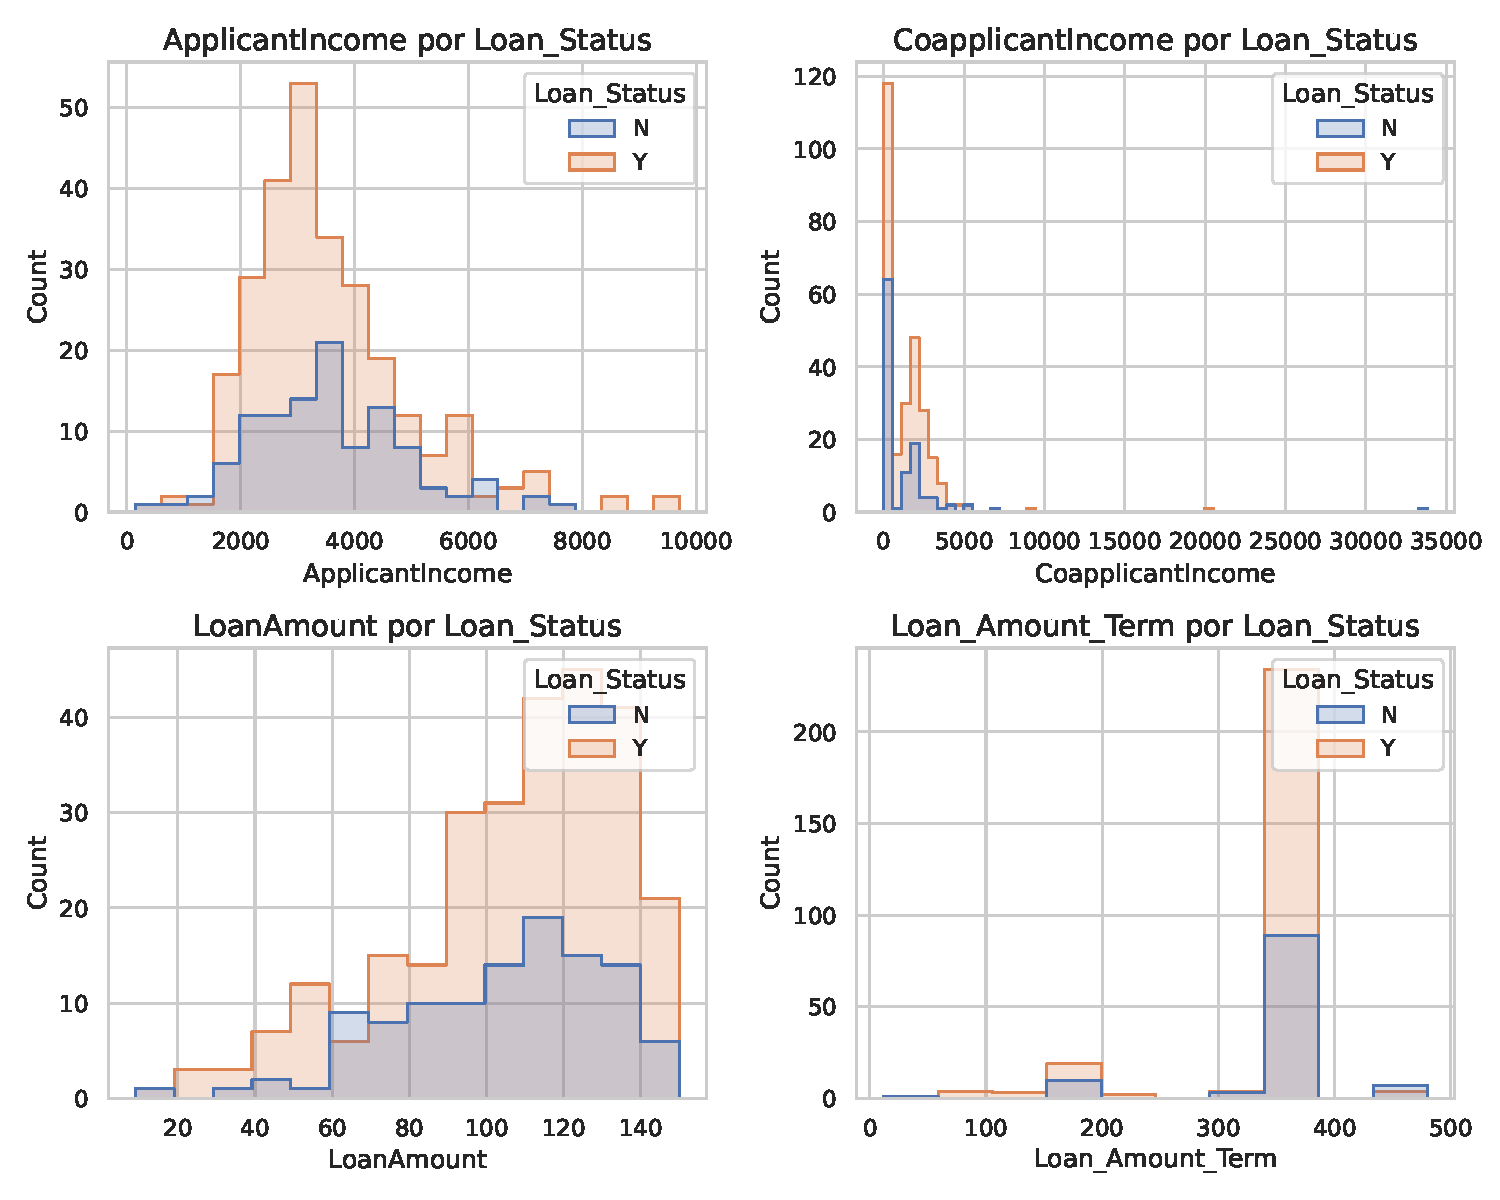
\includegraphics[scale=0.65]{Figures/histograma.pdf} \\
    Fonte: Elaborado pelo autor.
    \label{fig:1}
\end{figure}

Observando a Figura (\ref{fig:1}), nota-se que nenhum dos atributos segue uma distribuição normal. Embora, para a maioria dos modelos de classificação, isso não seja um requisito fundamental, ao contrário de muitos métodos estatísticos, é comum encontrar distribuições assimétricas. É notável que muitos dos valores dos atributos estão concentrados em torno da média ou mediana, acredita-se que as estatísticas reforçam o que é visto na Tabela (\ref{tab:1}), especialmente nos atributos \textit{CoapplicantIncome} e \textit{Loan\_Amount\_Term}. Como consequência, observamos a presença de valores que estão significativamente distantes dessa tendência, o que levanta a suspeita da existência de outliers. Esta suspeita será investigada na Figura (\ref{fig:2}), juntamente com o código utilizado, apresentado a seguir. Consulte o Código (12) para mais detalhes.
\begin{center}
\textbf{Código 12:} BoxPlot dos atributos numéricos.
\begin{minted}[linenos, fontsize=\footnotesize, bgcolor=bg]{python}
plt.figure(figsize=(10, 8), dpi=300)

i = 1
for column in loan_data.columns:
    if (loan_data[column].dtype == 'float64') or (loan_data[column].dtype == 'int64'):
        plt.subplot(2, 2, i) # Formato da matriz de gráficcos
        # Criando o gráfico
        ax = sns.boxplot(data=loan_data, y=column, x='Loan_Status', hue='Loan_Status')
        ax.set_title(f'{column} por Loan_Status', fontsize=14) # Título
        i += 1

plt.tight_layout()
plt.savefig('boxplot.pdf', format='pdf', dpi=300)
plt.show()\end{minted}
\end{center}

O gráfico da Figura (\ref{fig:2}) corresponde a saída do código acima.

\begin{figure}[H]
    \centering
    \caption{BoxPlots dos atributos numéricos.}
    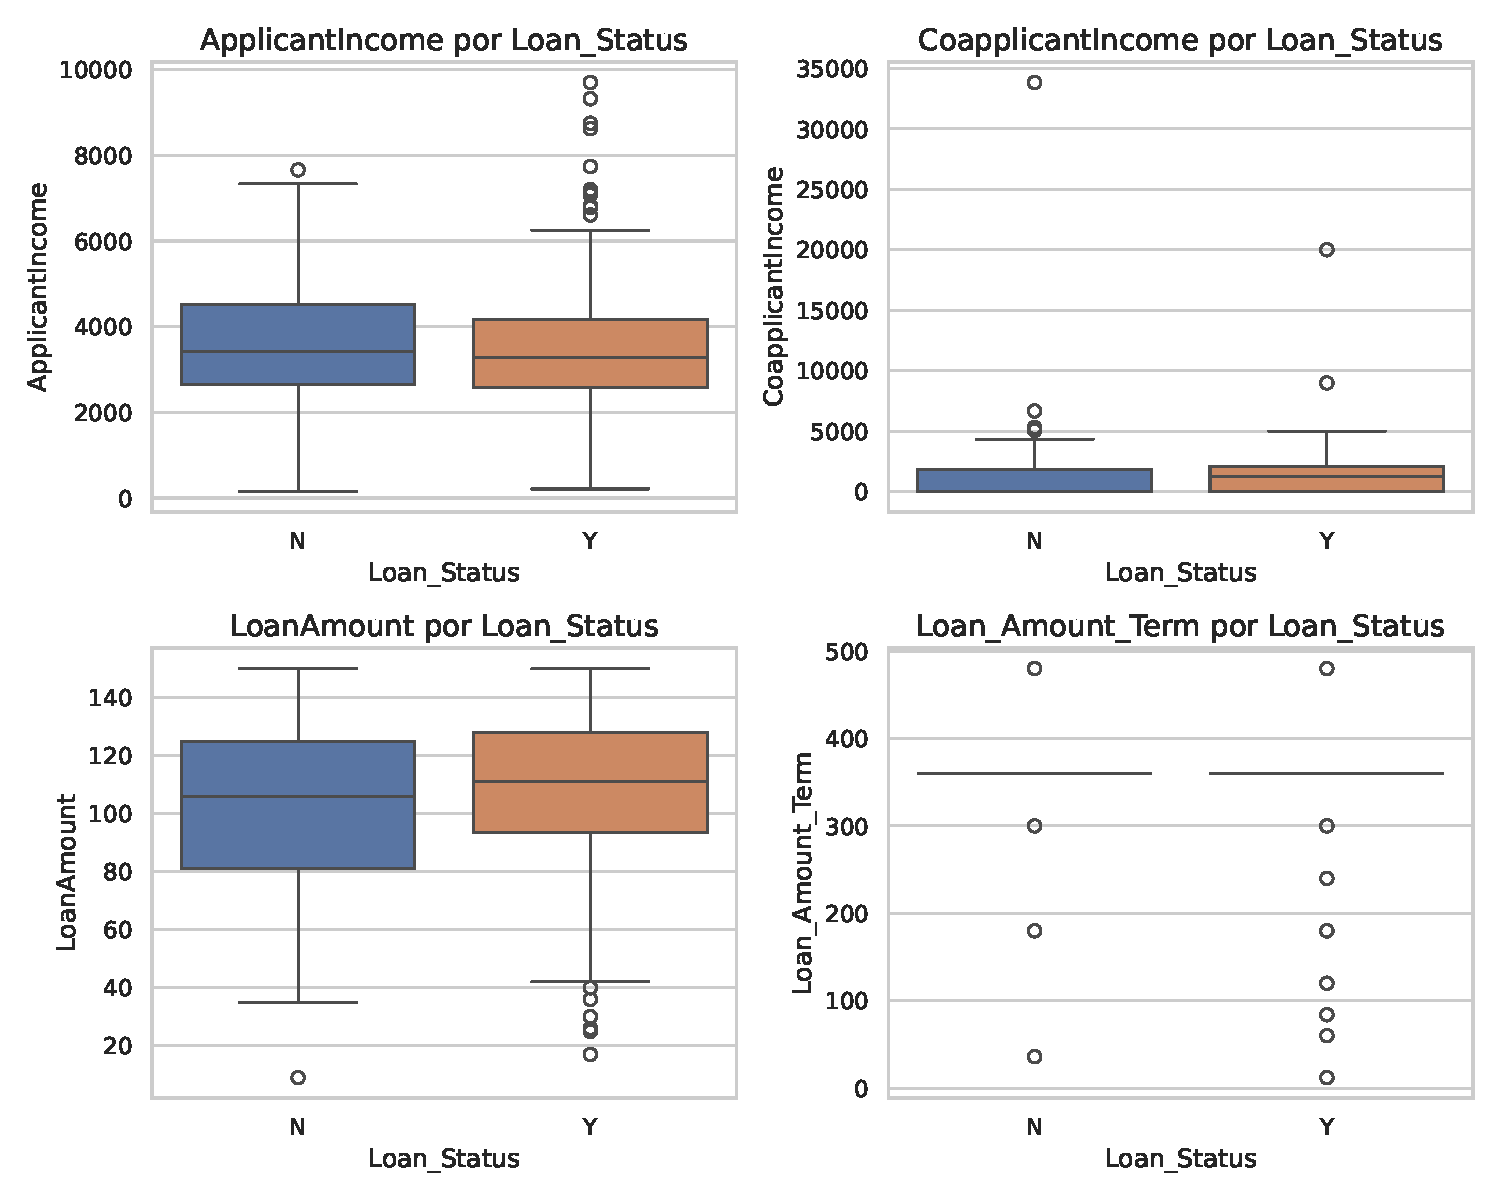
\includegraphics[scale=0.65]{Figures/boxplot.pdf} \\
    Fonte: Elaborado pelo autor.
    \label{fig:2}
\end{figure}

Analisando a Figura (\ref{fig:2}), podemos confirmar a suspeita levantada pela análise anterior da Figura (\ref{fig:1}): há presença de outliers em todos os gráficos e suas respectivas subcategorias. Além disso, observamos que a distribuição dos atributos numéricos é mais densa em praticamente todos os gráficos, com exceção dos montantes de empréstimo solicitados que foram recusados, onde o boxplot revela uma amplitude maior entre o primeiro e o terceiro quartil. Notamos que todas as medianas dos subgráficos são próximas, e as grandes diferenças residem nos valores extremos, que acabam por prejudicar a visualização. Apesar disso, optamos por manter a visualização com outliers (apesar de termos a opção de visualizar sem), pois já examinamos a distribuição por meio do Histograma na Figura (\ref{fig:1}), então é importante manter essas duas ferramentas nesse padrão para uma comparação consistente.

A seguir, apresentamos o Código (13) demonstrando a construção do Gráfico de Contagem, seguido pela Figura (\ref{fig:3}), resultado do Código (13), para uma análise das variáveis qualitativas do conjunto de dados.

\begin{center}
\textbf{Código 13:} Gráfico de contagem dos atributos não numéricos.
\begin{minted}[linenos, fontsize=\footnotesize, bgcolor=bg]{python}
plt.figure(figsize=(18, 8), dpi=300)

i = 1
for column in loan_data.columns:
    if loan_data[column].dtype == 'object':
        plt.subplot(2, 4, i)
        ax = sns.countplot(data=loan_data, x=column, hue='Loan_Status')
        ax.set_title(f'{column} por Loan_Status', fontsize=14)
        for num in [0, 1]:
          ax.bar_label(ax.containers[num], fontsize=10);
        i += 1

plt.tight_layout()
plt.savefig('countplot.pdf', format='pdf', dpi=300)
plt.show()
\end{minted}
\end{center}

O gráfico da Figura (\ref{fig:3}) é resultado do código a cima.

\begin{figure}[H]
    \centering
    \caption{Gráfico de contagem dos atributos não numéricos.}
    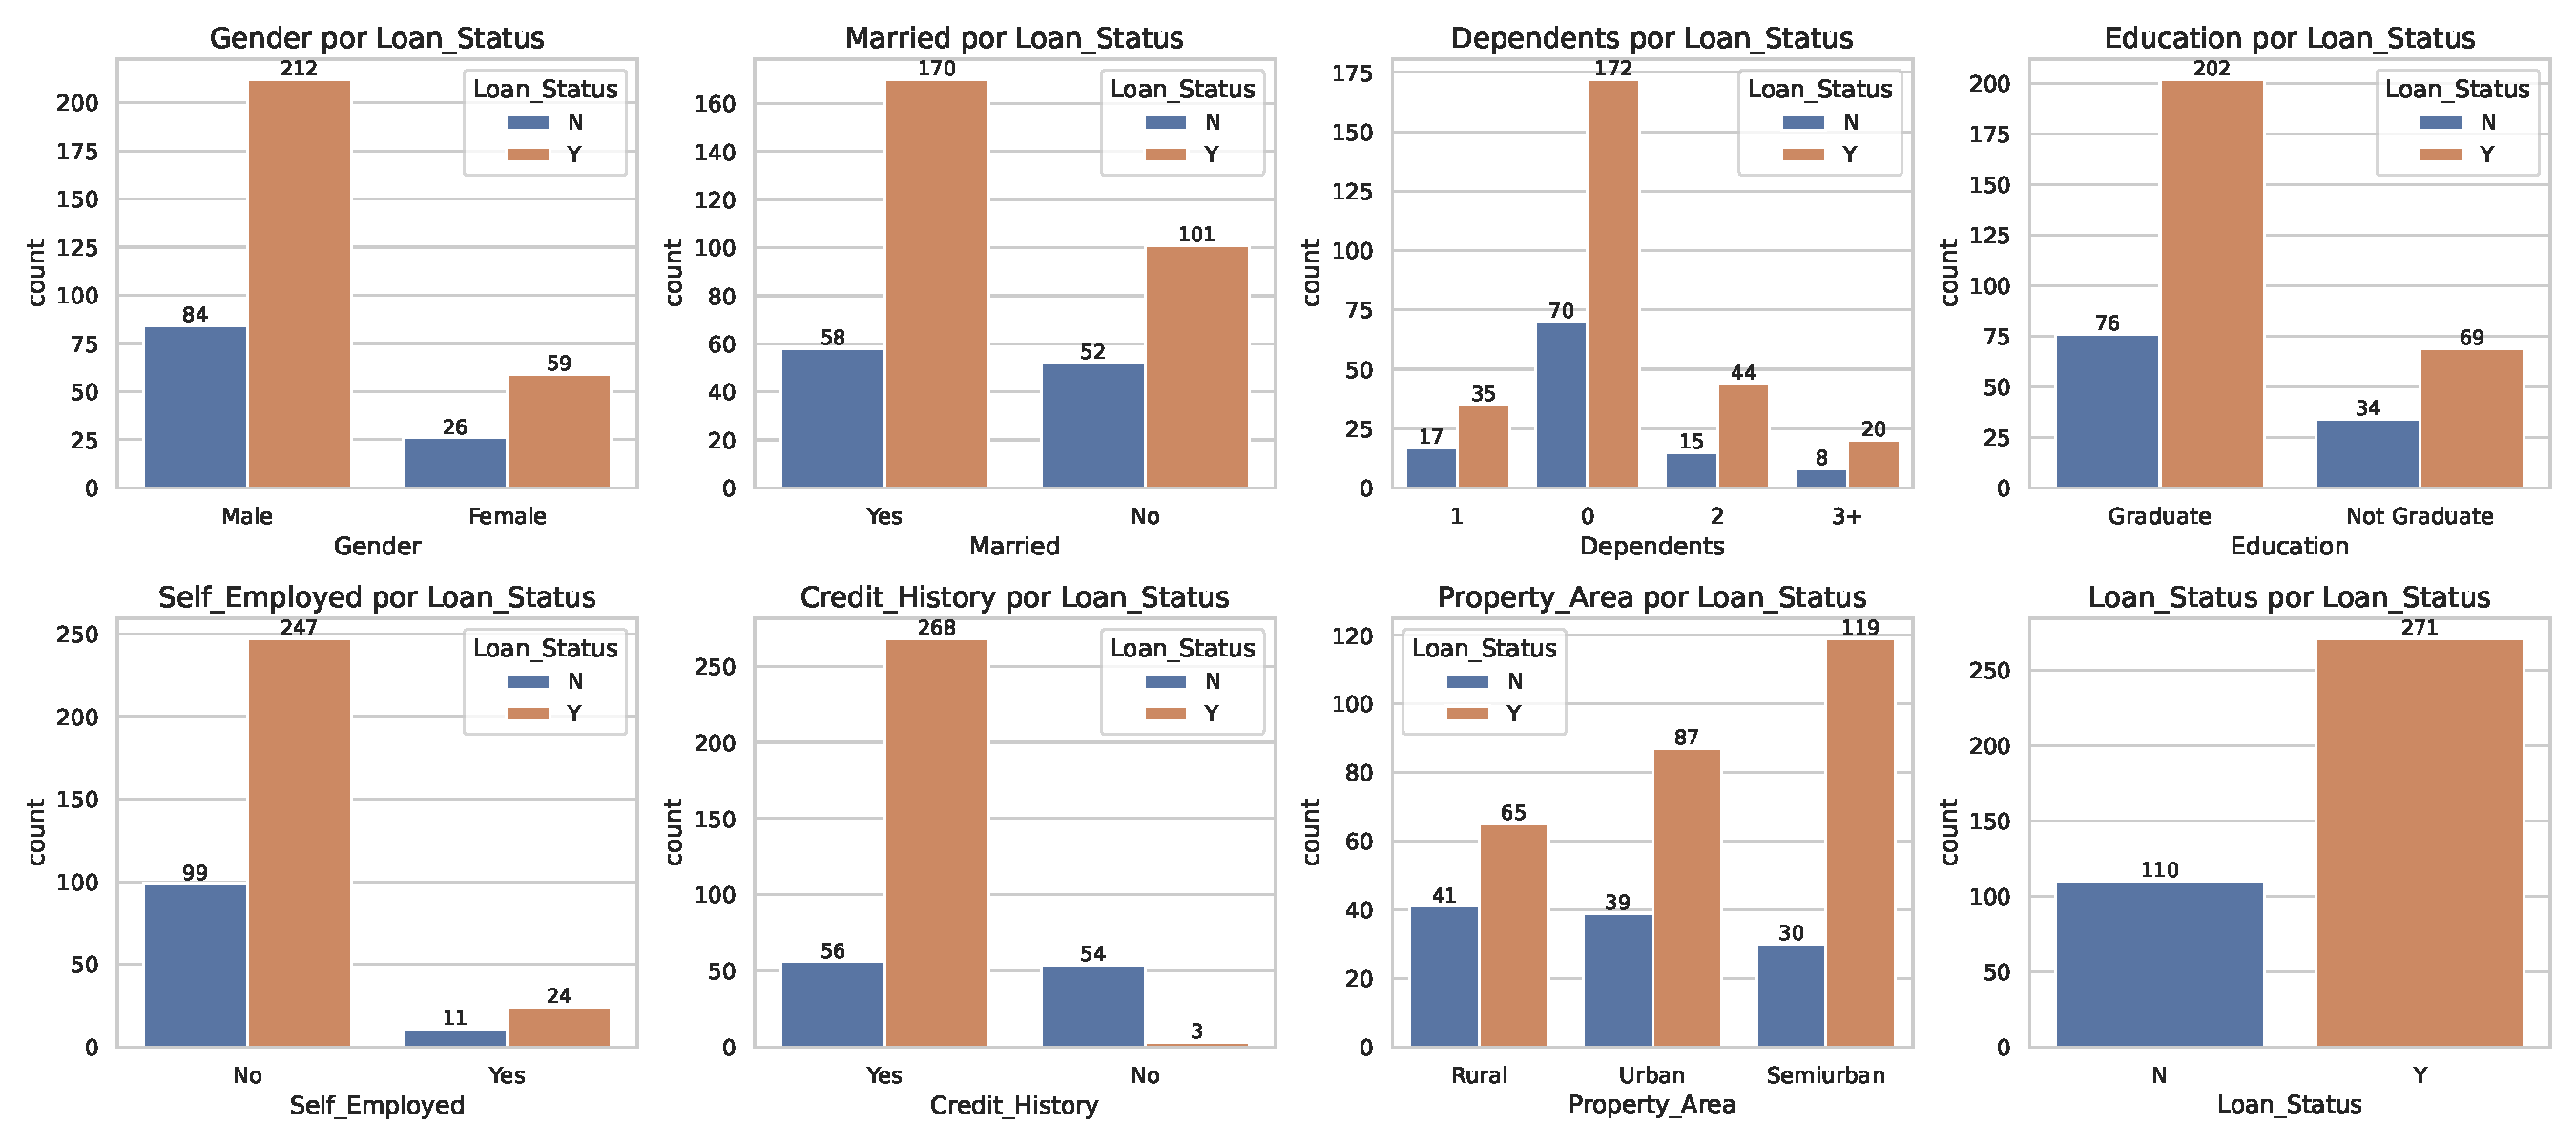
\includegraphics[scale=0.35]{Figures/countplot.pdf} \\
    Fonte: Elaborado pelo autor.
    \label{fig:3}
\end{figure}

O gráfico de contagem, também conhecido como gráfico de barras, é uma ferramenta extremamente útil para explorar atributos não numéricos, pois destaca claramente as diferenças entre esses atributos com base na variável alvo. Por exemplo, observa-se que a maioria dos registros no conjunto de dados teve seus empréstimos aprovados, representando cerca de 71,13\% do total. Graças ao gráfico de contagem, também pode-se discernir que a chance de um solicitante de empréstimo sem histórico de crédito satisfatório ter seu empréstimo aprovado é de aproximadamente 1,11\%. Por outro lado, a probabilidade de aprovação para solicitantes com histórico de crédito satisfatório é de 98,89\%. Com base nessas informações, é evidente que o atributo \textit{Credit\_History} deve ser altamente correlacionado com a variável alvo, tornando-se uma característica decisiva na decisão de aprovar ou não um empréstimo. Outros atributos também evidenciam claramente as diferenças entre os grupos com e sem aprovação de empréstimo, como os atributos \textit{Self\_Employed} e \textit{Dependents}. A probabilidade de aprovação para indivíduos não autônomos é significativamente maior do que para os autônomos, e a relação inversa se aplica ao número de dependentes do solicitante: quanto menor o número de dependentes, maior a probabilidade de aprovação do empréstimo. Ao analisarmos esses atributos isoladamente, eles parecem determinar claramente a aprovação do empréstimo. No entanto, ao considerarmos as combinações desses atributos, podemos esperar que os modelos tenha a necessidade de serem mais complexos e robustos. Pensando nisso, foram plotadas a Matriz de Correlação na Figura (\ref{fig:4}) e os Diagramas de Dispersão na Figura (\ref{fig:6}), com o objetivo de identificar essas possíveis relações mais complexas. Consulte o Código (14) para mais detalhes.
\begin{center}
\textbf{Código 14:} Matriz de Correlação de Pearson.
\begin{minted}[linenos, fontsize=\footnotesize, bgcolor=bg]{python}
plt.figure(figsize=(12, 6), dpi=300)
correlation =  loan_preprocessing.corr()

# plot da matriz de correlação
sns.heatmap(correlation, annot = True, fmt=".2f", linewidths=1.0)

plt.savefig('matrix_correlação.pdf', format='pdf', dpi=300)
plt.show()
\end{minted}
\end{center}

O gráfico da Figura (\ref{fig:4}) foi obtido a partir do código a cima.

\begin{figure}[H]
    \centering
    \caption{Matriz de Correlação de Pearson.}
    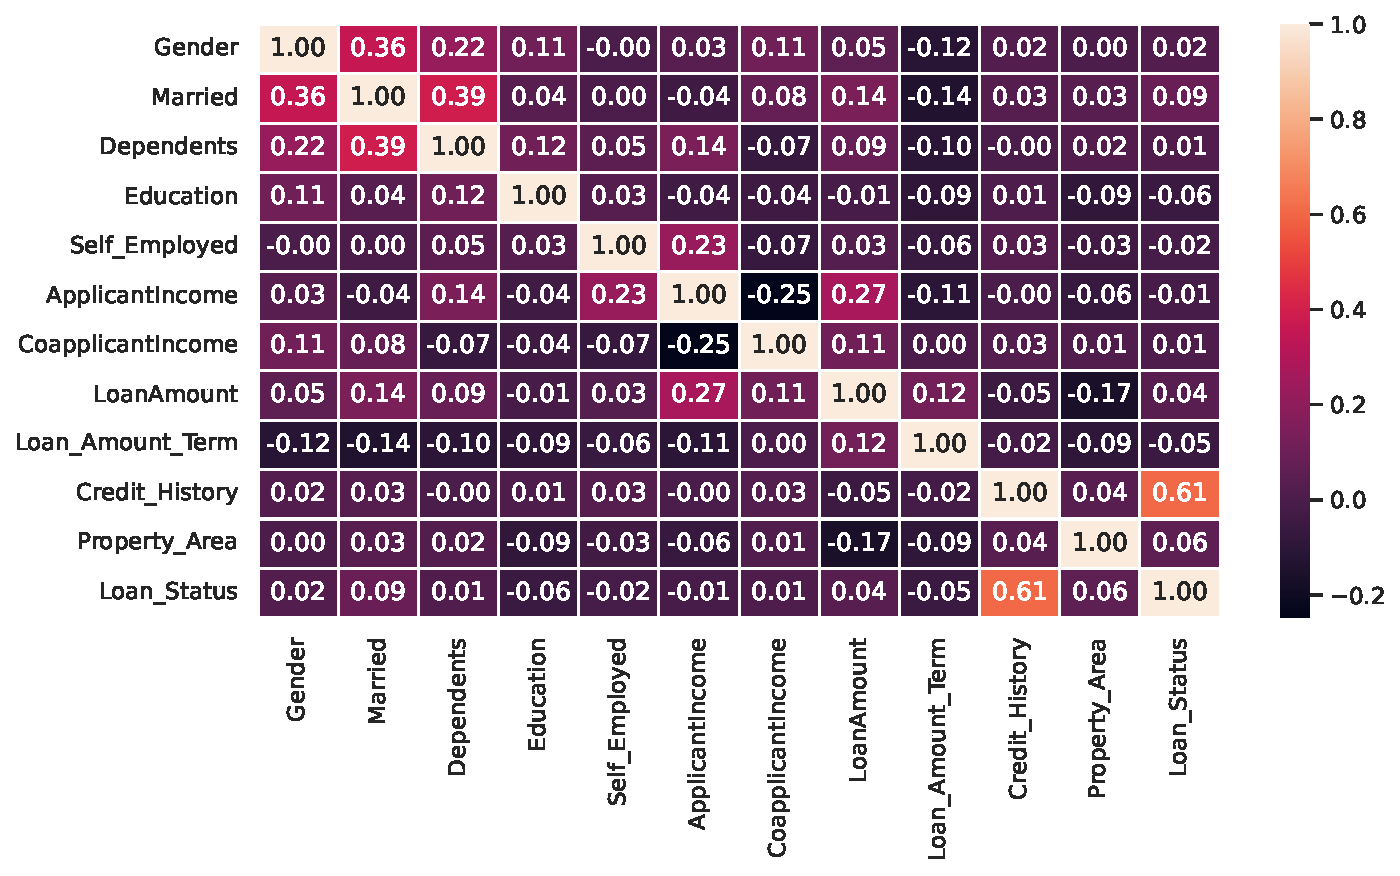
\includegraphics[scale=0.65]{Figures/pearson.pdf} \\
    Fonte: Elaborado pelo autor.
    \label{fig:4}
\end{figure}

Como discutido anteriormente e corroborado pela análise da Matriz de Correlação, observamos que o atributo mais fortemente correlacionado com nossa variável alvo é \textit{Credit\_History}, exibindo uma correlação moderadamente positiva. No entanto, é importante ressaltar que as demais variáveis podem apresentar correlações mais fracas, algumas até mesmo negativas, devido à natureza não linear das relações entre os atributos. Nesses casos, o Coeficiente de Correlação de Pearson pode não capturar com precisão tais relações. Portanto, decidimos recalculá-la utilizando o método de \textit{Spearman}, que é mais adequado para capturar correlações não lineares. Para obter mais detalhes sobre esse processo, consulte o Código (15).

\begin{center}
\textbf{Código 15:} Matriz de Correlação de Spearman.
\begin{minted}[linenos, fontsize=\footnotesize, bgcolor=bg]{python}
plt.figure(figsize=(10, 6), dpi=300)
correlation =  loan_preprocessing.corr(method='spearman')

# Plot da matriz de correlação
sns.heatmap(correlation, annot=True, fmt=".2f", linewidths=1.0)

# Ajustar a margem para permitir espaço extra para os rótulos do eixo x
plt.tight_layout()

# Salvar o gráfico em PDF com margens ajustadas
plt.savefig('spearman.pdf', format='pdf', dpi=300, bbox_inches='tight')
plt.show()
\end{minted}
\end{center}

A seguir a Matriz de Correlação de Spearman, veja a Figura (\ref{fig:5}).

\begin{figure}[H]
    \centering
    \caption{Matriz de Correlação de Spearman.}
    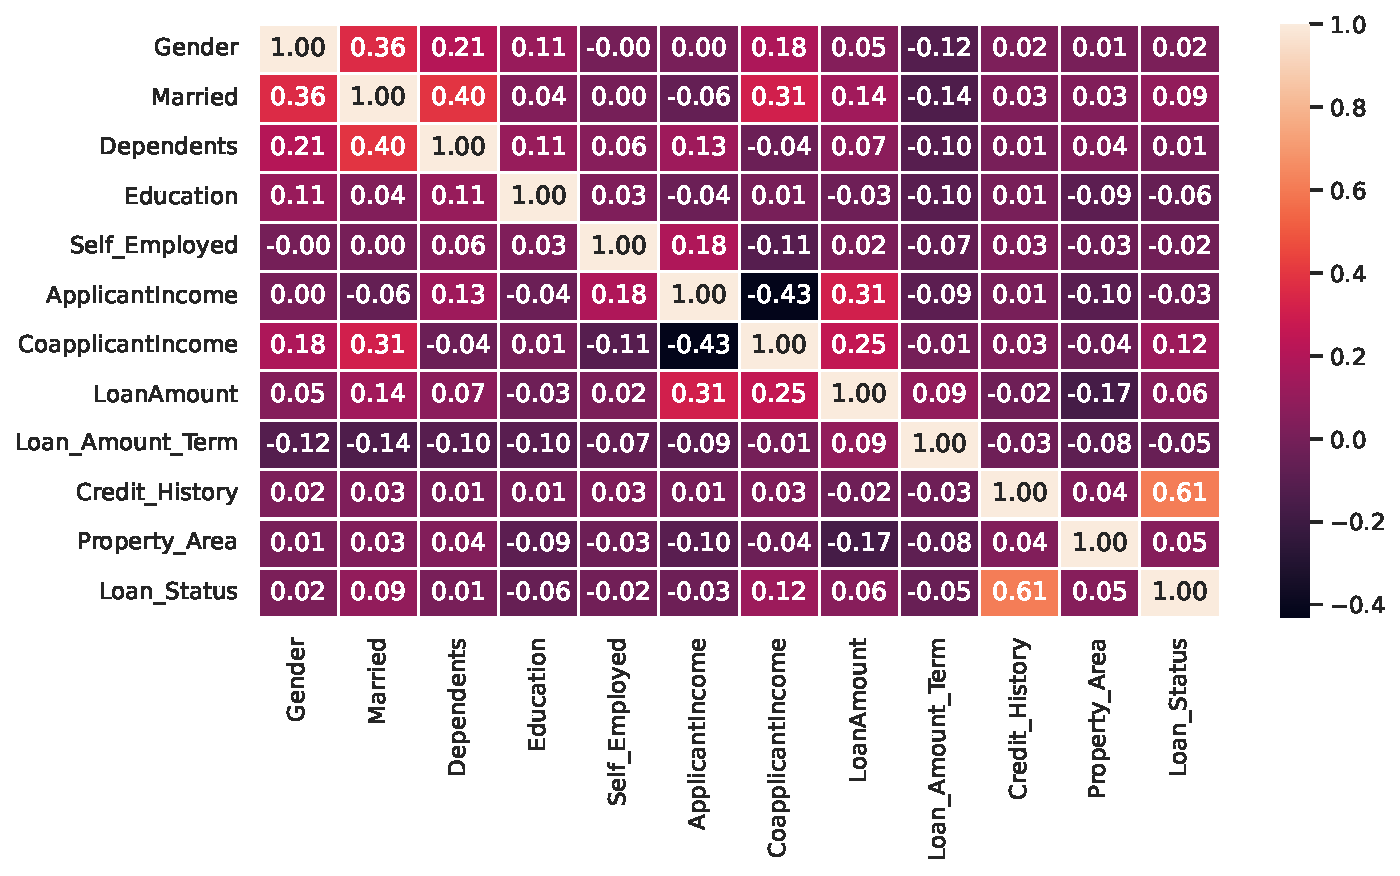
\includegraphics[scale=0.65]{Figures/spearman.pdf} \\
    \label{fig:5}
\end{figure}

Olhando só para as cores do mapa de calor, sem se atentar tanto aos números, podemos notar pequenas diferenças, mas nada de grande relevância. O atributo mais correlacionado ainda é \textit{Credit\_History}, com uma correlação classificada como moderada positiva. Agora, vamos analisar os Diagramas de Dispersão para verificar se a relação entre os atributos numéricos é linearmente separável e entender melhor como funciona essa relação, buscando tirar conclusões através de uma análise conjunta dos Diagramas com a Matriz de Correlação.
\begin{center}
\textbf{Código 16:} Diagramas de Dispersão.
\begin{minted}[linenos, fontsize=\footnotesize, bgcolor=bg]{python}
plt.figure(figsize=(12, 6), dpi=300)

sns.set(style='whitegrid')

sns.pairplot(loan_data, hue='Loan_Status', markers=['o', 'D'])

plt.savefig('pairplot.pdf', format='pdf', dpi=300)
plt.show()
\end{minted}
\end{center}

O gráfico da Figura (\ref{fig:6}) foi obtido a partir do código a cima.

\begin{figure}[H]
\selectlanguage{brazil}
    \centering
    \caption{Diagramas de Dispersão.}
    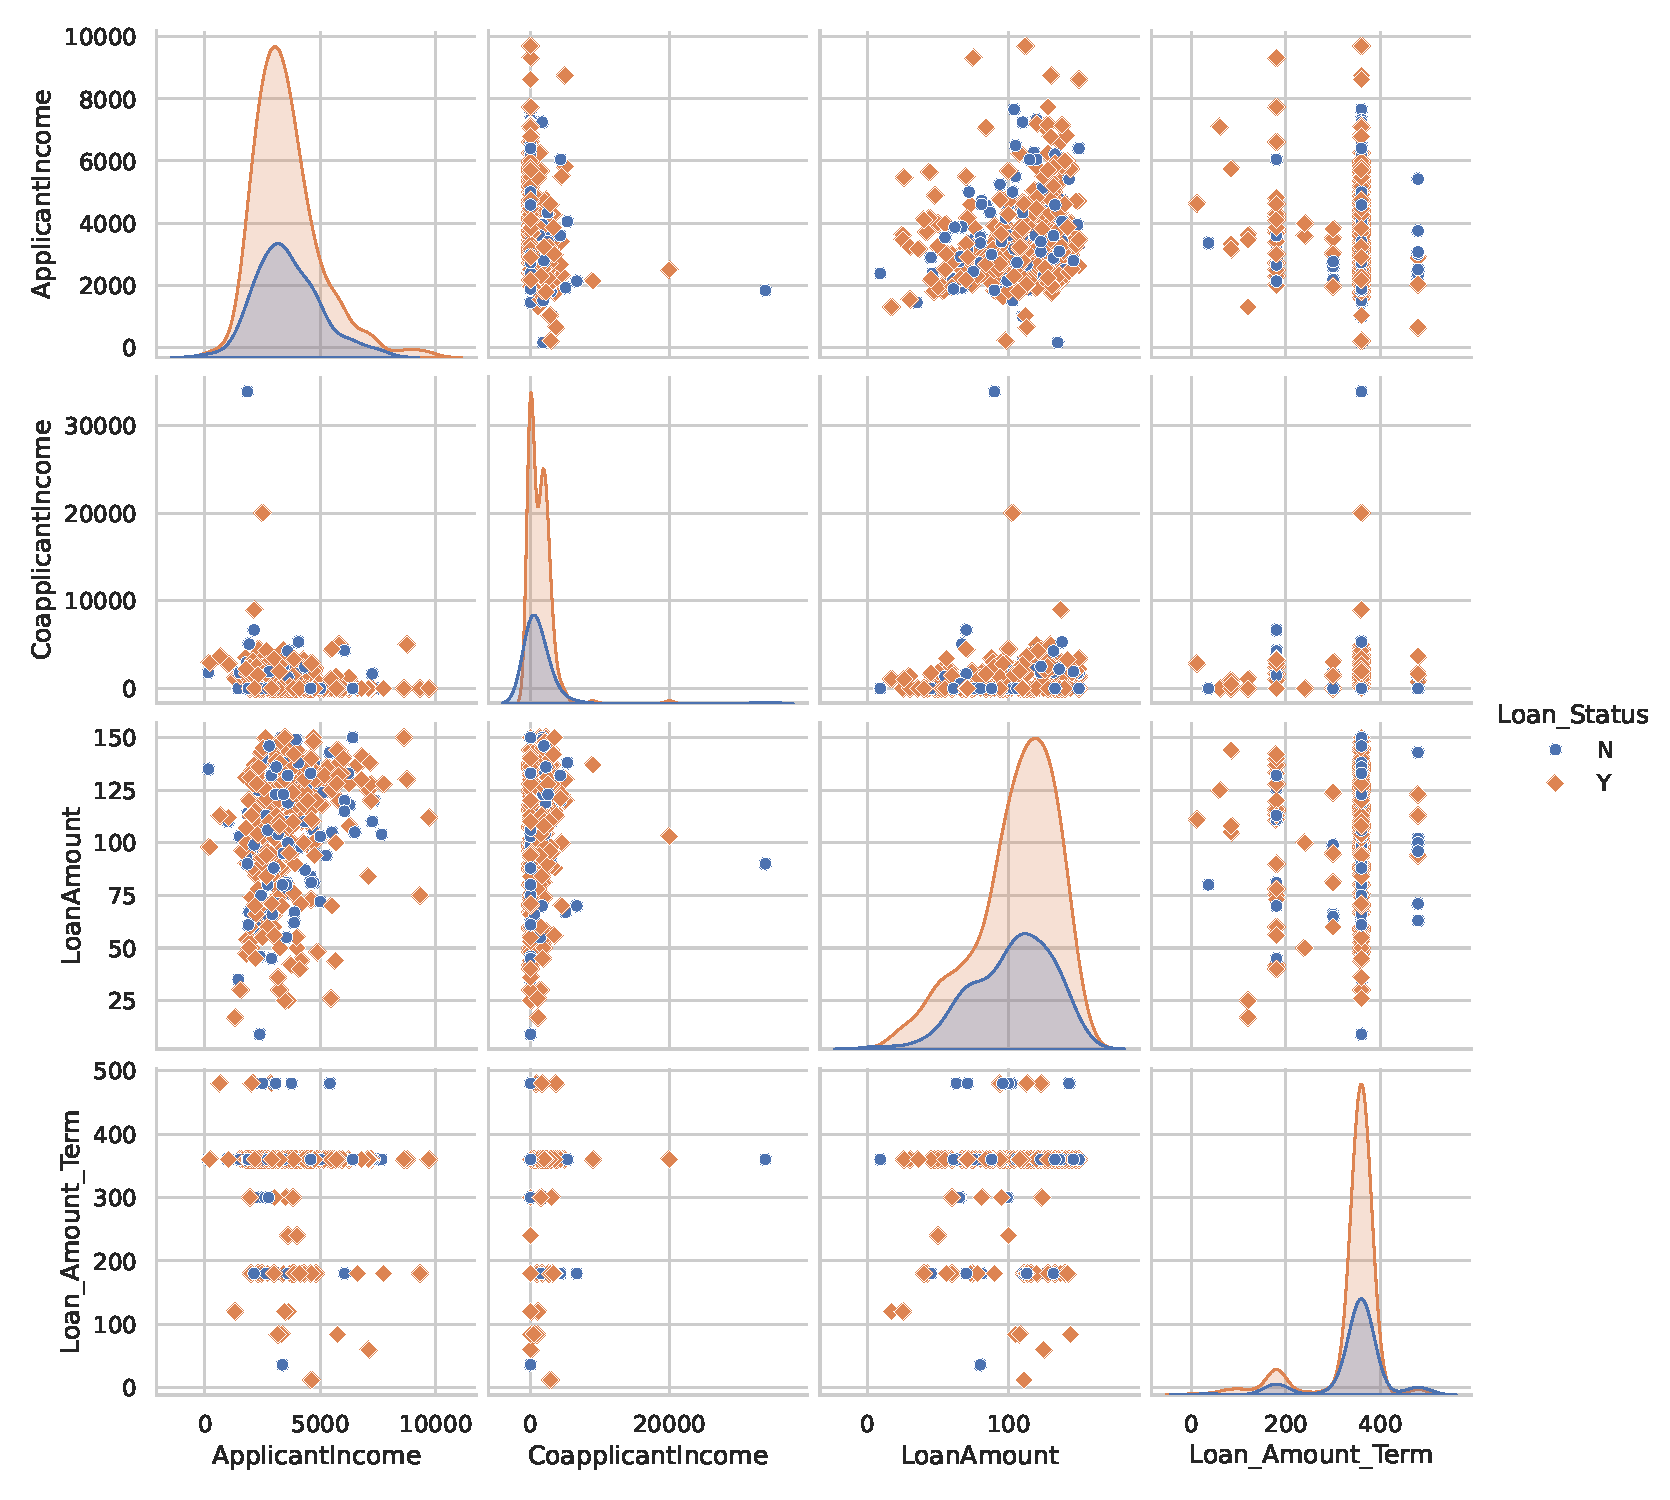
\includegraphics[scale=0.5]{Figures/pairplot.pdf} \\
    Fonte: Elaborado pelo autor.
    \label{fig:6}
\end{figure}

Observando os diagramas dos atributos numéricos, percebemos que nenhuma das relações é linearmente separável, e também não apresentam um padrão claro de relação. Com isso em mente, podemos antecipar que os modelos de classificação podem enfrentar dificuldades diante dessas características. Será necessário otimizar os hiperparâmetros em busca do melhor classificador.

Como considerações finais da Análise Exploratória de Dados, concluímos que os gráficos apresentados revelaram a distribuição dos dados, sua dispersão e os tipos de relações. Observamos que, em termos numéricos, as classes (empréstimo aprovado e empréstimo não aprovado) não são facilmente separáveis. Visualmente, um modelo baseado apenas nesses atributos numéricos seria muito complexo. No entanto, os atributos categóricos mostram uma melhor separação, embora apresentem uma complexidade própria que o modelo deve ser capaz de capturar. O dataset \textit{loan\_preprocessing} foi utilizado apenas para análise gráfica devido aos requisitos da função de plotagem gráfica da Matriz de Correlação, que exigia variáveis numéricas.

A próxima etapa será a separação do conjunto de dados (\textit{loan\_preprocessing}) em dados de treino e teste. Consulte a seção (\ref{section:3.3}) para mais detalhes.

\subsection{Separação do Conjunto de Dados} \label{section:3.3}
De acordo com Morettin \& Singer (2021):
\begin{quote}
    \textit{
    "O que hoje se entende como aprendizado com Estatística envolve duas classes de técnicas, denominadas \textbf{aprendizado supervisionado} e \textbf{aprendizado não supervisionado}. \\
    O \textbf{aprendizado supervisionado} está relacionado com metodologias desenvolvidas essencialmente para \textbf{previsão} e \textbf{classificação}. No âmbito da previsão, o objetivo é utilizar \textbf{variáveis preditoras} (sexo, classe social, renda, por exemplo) observadas em várias \textbf{unidades} (clientes de um banco, por exemplo) para “adivinhar” valores de uma \textbf{variável resposta} numérica (saldo médio, por exemplo) de novas unidades. O problema de classificação consiste em usar as variáveis preditoras para indicarem que categorias de uma variável resposta qualitativa (bons ou maus pagadores, por exemplo) as novas unidades estão classificadas."
    },
\end{quote}
para metodologias de classificação é fornecido ao algoritmo de aprendizado, ou indutor, um conjunto de exemplos de treinamento para os quais o rótulo da classe associada é conhecido. De forma geral, cada exemplo é descrito por um vetor de valores de características, ou atributos, e o rótulo da classe associada. O objetivo do algoritmo de indução é construir um classificador que possa determinar corretamente a classe de novos exemplos ainda não rotulados, ou seja, exemplos que não tenham o rótulo da classe \cite{monard2003conceitos}.

Visto as referências a cima, se torna de suma importância dividir o conjunto de dados em \textit{dados de treino} e \textit{dados de teste}. Já que a metodologia de aprendizado com estatística (veja \cite{morettin2021estatistica}) ou aprendizado de máquina (veja \cite{monard2003conceitos}) apontam e enfatizam esse tipo de procedimento, seja para previsão ou para classificação, que é o objetivo deste trabalho, classificar o status do empréstimo.

Vale lembrar que essa etapa poderia (assim como muitas outras) ser feitas em um bloco de código único, mas por fins de melhor entendimento da parte do leitor, essa etapa foi dividida em 3 (três) blocos de código.

Antes de apresentarmos os códigos de separação do conjunto de dados, vamos entender melhor um parâmetro que aparece em grande parte das funções que iremos utilizar posteriormente. Chamado de \textit{random\_state}, que traduzido do inglês é \textit{estado aleatório}, é comumente encontrado em várias funções de bibliotecas do Python, como scikit-learn e NumPy, bibliotecas essas que estão sendo usadas nesse trabalho, que envolvem aleatoriedade ou geração de números aleatórios. Ele controla a aleatoriedade reproduzível ao executar o código, garantindo que os resultados sejam consistentes em diferentes execuções. Para uma melhor compreensão da geração de números aleatórios em Python, veja \cite{python-random}.

No código a seguir, iremos setar a semente, ou seja, definir um número  que será usado em todas as funções que apresentem o parâmetro \textit{random\_state} e definir o tamanho dos \textit{dados de treino}. Veja o Código (17) a seguir.
\begin{center}
\textbf{Código 17:} Definição da semente usada e do tamanho do conjunto de treino.
\begin{minted}[linenos, fontsize=\footnotesize, bgcolor=bg]{python}
size = 0.8 # tamanho do conjunto de treino
seed = 16 # semente
\end{minted}
\end{center}

No código a cima, o objeto semente pode ser variado pelo número inteiro de seu interesse, não há nenhum padrão para este número, porém o mais popular é a semente de número 42 por  motivos que eu não irei dizer aqui (caso tenha curiosidade, veja \cite{random42}). Não recomenda-se alteração no tamanho dos conjuntos apesar de não haver algo que impeça (alguma regra específica, por exemplo) de alterar, entretanto 80\% dos dados para treino e 20\% para testes quase sempre nos dão um bom resultado porém, as vezes seja interessante a aumentar o conjunto de teste e consequentemente diminuir o de treino ou vice e versa, o que seja mais adequado para o seu problema. Sendo questões de escolha do pesquisador.

\begin{center}
\textbf{Código 18:} Separando a matriz de atributos da coluna alvo.
\begin{minted}[linenos, fontsize=\footnotesize, bgcolor=bg]{python}
X = loan_preprocessing.drop(columns='Loan_Status') # Matriz de Atributos
y = loan_preprocessing['Loan_Status'] # Coluna Alvo
\end{minted}
\end{center}

Após a separação da matriz de atributos da coluna alvo, serão divididos os conjuntos $X$ e $y$ definidos acima para treinamento e para testes.  Veja o Código (19).

\begin{center}
\textbf{Código 19:} Separação do conjunto de dados em treino e teste.
\begin{minted}[linenos, fontsize=\footnotesize, bgcolor=bg]{python}
X_train, X_test, y_train, y_test = train_test_split(X, y,
                                                    train_size = size,
                                                    random_state = seed)
\end{minted}
\end{center}

Com isso, é dado fim a etapa de \textit{Separação do Conjunto de Dados em Treino e Teste} e inicia-se a etapa de desenvolvimento de modelos. Veja a seção (\ref{section:3.4})

\subsection{Desenvolvimento de Modelos} \label{section:3.4}
Nesta fase, adentra-se à etapa de \textit{Classificação}, a qual compreende as subetapas de \textit{Modelos Iniciais}, \textit{Variação de Hiperparâmetros} e \textit{Modelos Finais}. Aqui, serão iniciados os modelos e exploradas diferentes combinações de hiperparâmetros em busca da configuração mais eficaz e, por fim, será feito o ajuste desses novos hiperparâmetros nos modelos finais, respectivamente. Inicia-se o processo de examinação dos Modelos Iniciais na seção (\ref{section:3.4.1}).

Uma observação importante para o estimado leitor é que não se entrará em detalhes sobre cada hiperparâmetro e sua influência em cada função, uma vez que tais informações estão disponíveis na documentação da biblioteca (consulte \cite{sklearn}).

\subsubsection{Modelos Iniciais} \label{section:3.4.1}
Os códigos desta etapa serão resumidos em poucos blocos, uma vez que se trata da criação dos objetos modelos e do treinamento dos mesmos, utilizando no entanto, os hiperparâmetros padrão das funções dos objetos classificadores. Consulte o Código (20) para mais detalhes.
\begin{center}
\textbf{Código 20:} Inicialização e Treinamento dos Modelos Iniciais.
\begin{minted}[linenos, fontsize=\footnotesize, bgcolor=bg]{python}
# Árvore de Decisão (Decision Tree)
# Criação e inicialização do modelo
first_tree = DecisionTreeClassifier(random_state = seed)

# Ajuste (Treinamento)
first_tree.fit(X_train, y_train)

# kNN (kNeighbors)
# Criação e inicialização do modelo
first_kNN = KNeighborsClassifier()

# Ajuste (Treinamento)
first_kNN.fit(X_train, y_train)

# Naive Bayes Gaussiano (GaussianNB)
# Criação e inicialização do modelo
first_gnb = GaussianNB(var_smoothing = 1e-5)

# Ajuste (Treinamento)
first_gnb.fit(X_train, y_train)

# Regrssão Logística ()
# Criação e inicialização do modelo
first_lg = LogisticRegression(tol = 1e-5, random_state = seed)

# Ajuste (Treinamento)
first_lg.fit(X_train, y_train)

# Redes Neurais (NeuralNetworks)
# Criação e inicialização do modelo
first_mlp = MLPClassifier(alpha = 1e-5, random_state = seed)

# Ajuste (Treinamento)
first_mlp.fit(X_train, y_train)

# SVM (Support Vector Machine)
# Criação e inicialização do modelo
first_svm = SVC(tol = 1e-5, random_state = seed)

# Ajuste (Treinamento)
first_svm.fit(X_train, y_train)

# Métodos de Assembleia (Methods in Assembly) # RandomForest (Florestas Aleatórias)
# Criação e inicialização do modelo
first_randomforest = RandomForestClassifier(random_state = seed)

# Ajuste (Treinamento)
first_randomforest.fit(X_train, y_train)

# Métodos de Assembleia (Methods in Assembly) # Método de classificação VotingClassifier
# Criação e inicialização do modelo
classifiers = [('DecisionTre', first_tree), ('kNN', first_kNN), ('GaussianNB', first_gnb),
               ('LogisticRegression', first_lg), ('NeuralNetworks', first_mlp),
               ('SVM', first_svm), ('RandomForest', first_randomforest)]
first_voting = VotingClassifier(estimators = classifiers)

# Ajuste (Treinamento)
first_voting.fit(X_train, y_train)
\end{minted}
\end{center}

No Código (20), iniciamos a classificação, criamos os objetos modelos e realizamos o treinamento. Após a criação e treinamento dos modelos, realizamos testes para prever o status de empréstimo utilizando a matriz de atributos separada para testes. Consulte o Código (21) para mais detalhes.

\begin{center}
\textbf{Código 21:} Teste dos Modelos Iniciais.
\begin{minted}[linenos, fontsize=\footnotesize, bgcolor=bg]{python}
# Teste dos Modelos
first_treeP = first_tree.predict(X_test) # Árvore de Decisão
first_kNNP = first_kNN.predict(X_test) # kNN
first_gnbP = first_gnb.predict(X_test) # GaussianNB
first_lgP = first_lg.predict(X_test) # Regressão Logística
first_mlpP = first_mlp.predict(X_test) # Redes Neurais
first_svmP = first_svm.predict(X_test) # SVM
first_randomforestP = first_randomforest.predict(X_test) # Assembly: RandomForest
first_votingP = first_voting.predict(X_test) # Assembly: VotingClassifier
\end{minted}
\end{center}

Os resultados de tais predições foram dispostos na seção (\ref{section:4.1.1}), já sendo a etapa de avaliação de modelos.

Se torna adequado falar que, em alguns modelos foram definidos hiperparâmetros além do \textit{default} e/ou \textit{random\_state} entretanto, esses hiperparâmetros foram definidos previamente pois, não ocorrerá a variação deles, logo, são hiperparâmetros fixos e por isso já foram definidos.

\subsubsection{Variação de Hiper Parâmetros}
Esta etapa destina-se a averiguar se há alguma outra combinação (além da padrão) que resulte em uma melhor acurácia para nosso conjunto de dados e objetivo. Foi desenvolvida uma estrutura de código única na qual apenas as peculiaridades de cada classificador foram alteradas.

Nesta etapa, é importante lembrar que existe uma função específica para esse tipo de varredura e averiguação. No entanto, devido às limitações de memória (RAM) do ambiente de desenvolvimento integrado (IDE Google Colaoratory) da linguagem utilizada (Python), optamos por criar essa estrutura de código, a qual pôde ser processada com sucesso.

Para esta etapa, foram selecionados os seguintes modelos: \textit{Árvore de Decisão}, \textit{kNN}, \textit{Regressão Logística}, \textit{Redes Neurais}, \textit{SVM} e \textit{Florestas Aleatórias}. A escolha desses classificadores foi baseada no critério de que a variação de seus hiperparâmetros teria um impacto significativo nos resultados. Cada variação realizada será acompanhada pelo código correspondente, disponível nos Códigos (22, 23, 24, 25, 26, 27). Os resultados de cada execução serão apresentados na Tabela (\ref{tab:3}).

\begin{center}
\textbf{Código 22:} Variação dos Hiper Parâmetros do classificador de Árvore de Decisão.
\begin{minted}[linenos, fontsize=\footnotesize, bgcolor=bg]{python}
# Variação dos Hiper Parâmetros do classificador de Árvore de Decisão
# Definir os valores para cada parâmetro
criterion = ['gini', 'entropy', 'log_loss']
splitter = ['best', 'random']
max_features = ['auto', 'sqrt', 'log2', None]

# Criar a lista de todas as combinações possíveis
parameters = list(product(criterion, splitter, max_features))

# Listas das acurácias obtidas
accuracy_list = []
for param in parameters:
    tree = DecisionTreeClassifier(criterion=param[0],
                                  splitter=param[1],
                                  max_features=param[2],
                                  random_state=seed)
    tree.fit(X_train, y_train)
    predict = tree.predict(X_test)
    accuracy = accuracy_score(predict, y_test) * 100
    accuracy_list.append(accuracy)


# Classificar as acurácias em ordem decrescente
sorted_acuracy = pd.Series(data=accuracy_list).sort_values(ascending=False)

# Obter a melhor acurácia e seus parâmetros correspondentes
best_acuracy = sorted_acuracy.iloc[0]
best_parameters_tree = parameters[sorted_acuracy.index[0]]

# Exibir resultados
print(f'O conjunto de parâmetros com maior acurácia ({best_acuracy:.2f}%) foi:')
print(best_parameters_tree)
\end{minted}
\end{center}

\begin{center}
\textbf{Código 23:} Variação dos Hiper Parâmetros do classificador de kNN.
\begin{minted}[linenos, fontsize=\footnotesize, bgcolor=bg]{python}
# Variação dos Hiper Parâmetros do classificador de kNN
# Definir os valores/intervalos para cada parâmetro
n_neighbors = range(3, 11)
weights = ['uniform', 'distance']
algorithm = ['auto', 'ball_tree', 'kd_tree', 'brute']
leaf_size = range(10, 101, 10)
metric = ['euclidean', 'manhattan', 'minkowski']

# Criar a lista de todas as combinações possíveis
parameters = list(product(n_neighbors, weights, algorithm, leaf_size, metric))

# Listas das acurácias obtidas
accuracy_list = []
for param in parameters:
  kNN = KNeighborsClassifier(n_neighbors=param[0],
                             weights=param[1],
                             algorithm=param[2],
                             leaf_size=param[3],
                             metric=param[4])
  kNN.fit(X_train, y_train)
  predict = kNN.predict(X_test)
  accuracy = accuracy_score(predict, y_test) * 100
  accuracy_list.append(accuracy)

# Classificar as acurácias em ordem decrescente
sorted_acuracy = pd.Series(data=accuracy_list).sort_values(ascending=False)

# Obter a melhor acurácia e seus parâmetros correspondentes
best_acuracy = sorted_acuracy.iloc[0]
best_parameters_kNN = parameters[sorted_acuracy.index[0]]

# Exibir resultados
print(f'O conjunto de parâmetros com maior acurácia ({best_acuracy:.2f}%) foi:')
print(best_parameters_kNN)
\end{minted}
\end{center}

\begin{center}
\textbf{Código 24:} Variação dos Hiper Parâmetros do classificador de Regressão Logística.
\begin{minted}[linenos, fontsize=\footnotesize, bgcolor=bg]{python}
# Variação dos Hiper Parâmetros do classificador de Regressão Logística
# Definir os valores para cada parâmetro
C = [0.001, 0.01, 0.1, 1, 10, 100]
solver = ['lbfgs', 'liblinear', 'newton-cg', 'sag', 'saga']
max_iter = range(100, 1001, 100)
class_weight = ['balanced', None]

# Criar a lista de todas as combinações possíveis
parameters = list(product(C, solver, max_iter, class_weight))

# Listas das acurácias obtidas
accuracy_list = []
for param in parameters:
    lg = LogisticRegression(C=param[0],
                            solver=param[1],
                            max_iter=param[2],
                            class_weight=param[3],
                            tol=1e-5, random_state=seed)
    lg.fit(X_train, y_train)
    predict = lg.predict(X_test)
    accuracy = accuracy_score(predict, y_test) * 100
    accuracy_list.append(accuracy)

# Classificar as acurácias em ordem decrescente
sorted_accuracy = pd.Series(data=accuracy_list).sort_values(ascending=False)

# Obter a melhor acurácia e seus parâmetros correspondentes
best_accuracy = sorted_accuracy.iloc[0]
best_parameters_lg = parameters[sorted_accuracy.index[0]]

# Exibir resultados
print(f'O conjunto de parâmetros com maior acurácia ({best_accuracy:.2f}%) foi:')
print(best_parameters_lg)
\end{minted}
\end{center}

\begin{center}
\textbf{Código 25:} Variação dos Hiper Parâmetros do classificador de Redes Neurais.
\begin{minted}[linenos, fontsize=\footnotesize, bgcolor=bg]{python}
# Variação dos Hiper Parâmetros do classificador de Redes Neurais
# Definir os valores/intervalos para cada parâmetro
n = range(3, 104, 25)
m = range(1, 102, 25)
activation = ['identity', 'logistic', 'tanh', 'relu']
solver = ['lbfgs', 'sgd', 'adam']
iter = range(250, 1001, 250)
# Criar a lista de todas as combinações possíveis
parameters = list(product(n, m, activation, solver, iter))

# Número de amostras
#n_samples = 200
# Amostras
#samples = random.sample(parameters, n_samples)

# Listas das acurácias obtidas
accuracy_list = []
for param in parameters: # caso opte pelo código comentado: for param in samples:
    mlp = MLPClassifier(hidden_layer_sizes=(param[0], param[1]),
                        activation=param[2],
                        solver=param[3],
                        max_iter=param[4],
                        alpha=1e-5,
                        random_state=seed)
    mlp.fit(X_train, y_train)
    predict = mlp.predict(X_test)
    accuracy = accuracy_score(predict, y_test) * 100
    accuracy_list.append(accuracy)

# Classificar as acurácias em ordem decrescente
sorted_accuracy = pd.Series(data=accuracy_list).sort_values(ascending=False)

# Obter a melhor acurácia e seus parâmetros correspondentes
best_accuracy = sorted_accuracy.iloc[0]
best_parameters_mlp = parameters[sorted_accuracy.index[0]]

# Exibir resultados
print(f'O conjunto de parâmetros com maior acurácia ({best_accuracy:.2f}%) foi:')
print(best_parameters_mlp)
\end{minted}
\end{center}

\begin{center}
\textbf{Código 26:} Variação dos Hiper Parâmetros do classificador de SVM.
\begin{minted}[linenos, fontsize=\footnotesize, bgcolor=bg]{python}
# Variação dos Hiper Parâmetros do classificador de SVM
# Definir os valores/intervalos para cada parâmetro
kernel = ['linear', 'poly', 'rbf', 'sigmoid']
gamma = ['scale', 'auto']
probability = [True, False]
class_weight = ['balanced', None]

# Criar a lista de todas as combinações possíveis
parameters = list(product(kernel, gamma, probability, class_weight))

# Listas das acurácias obtidas das amostras
accuracy_list = []
for param in parameters:
  svm = SVC(kernel=param[0],
            gamma=param[1],
            probability=param[2],
            class_weight=param[3],
            tol=1e-5,
            random_state=seed)
  svm.fit(X_train, y_train)
  predict = svm.predict(X_test)
  accuracy = accuracy_score(predict, y_test) * 100
  accuracy_list.append(accuracy)

# Classificar as acurácias em ordem decrescente
sorted_acuracy = pd.Series(data=accuracy_list).sort_values(ascending=False)

# Obter a melhor acurácia e seus parâmetros correspondentes
best_acuracy = sorted_acuracy.iloc[0]
best_parameters_svm = parameters[sorted_acuracy.index[0]]

# Exibir resultados
print(f'O conjunto de parâmetros com maior acurácia ({best_acuracy:.2f}%) foi:')
print(best_parameters_svm)
\end{minted}
\end{center}

\begin{center}
\textbf{Código 27:} Variação dos Hiper Parâmetros do classificador de Florestas Aleatórias.
\begin{minted}[linenos, fontsize=\footnotesize, bgcolor=bg]{python}
# Variação dos Hiper Parâmetros do classificador de RandomForest (Florestas Aleatórias)
# Definir os valores/intervalos para cada parâmetro
n_estimators = range(100, 1000, 100)
criterion = ['gini', 'entropy', 'log_loss']
max_features = ['auto', 'sqrt', 'log2', None]

# Criar a lista de todas as combinações possíveis
parameters = list(product(n_estimators, criterion, max_features))

# Listas das acurácias obtidas das amostras
accuracy_list = []
for param in parameters:
  randomforest = RandomForestClassifier(n_estimators=param[0],
                                        criterion=param[1],
                                        max_features=param[2],
                                        random_state=seed)
  randomforest.fit(X_train, y_train)
  predict = randomforest.predict(X_test)
  accuracy = accuracy_score(predict, y_test) * 100
  accuracy_list.append(accuracy)

# Classificar as acurácias em ordem decrescente
sorted_acuracy = pd.Series(data=accuracy_list).sort_values(ascending=False)

# Obter a melhor acurácia e seus parâmetros correspondentes
best_acuracy = sorted_acuracy.iloc[0]
best_parameters_rf = parameters[sorted_acuracy.index[0]]

# Exibir resultados
print(f'O conjunto de parâmetros com maior acurácia ({best_acuracy:.2f}%) foi:')
print(best_parameters_rf)
\end{minted}
\end{center}

Veja a Tabela (\ref{tab:3}) que consta os modelos, a melhor combinação de hiperparâmetros e a acurácia obtida de cada modelo.

\begin{table}[H]
    \centering
    \caption{Resultados da Variação de Parâmetros dos modelos.}
    \begin{tabular}{c|c|c}
    \hline
    Classificador & Conjunto de Parâmetros & Acurácia \\
    \hline
    \multirow{3}{*}{Árvore de Decisão} & criterion: 'log-loss' & \multirow{3}{*}{92,21\%} \\
     & splitter: 'random' & \\
     & max\_features: 'None' & \\
    \hline
    \multirow{5}{*}{kNN} & n\_neighbors: 6 & \multirow{5}{*}{87,01\%} \\
     & weights: 'uniform' & \\
     & algorithm: 'kd\_tree' & \\
     & leaf\_size: 10 & \\
     & metric: 'manhattan' & \\
    \hline
    \multirow{4}{*}{Regressão Logística} & C: 100 & \multirow{4}{*}{89,61\%} \\
     & solver: 'saga' & \\
     & max\_iter: 1000 & \\
     & class\_weight: None & \\
    \hline
    \multirow{4}{*}{Redes Neurais} & hidden\_layer\_sizes: (3, 26) & \multirow{4}{*}{90,91\%} \\
     & activation: 'logistic' & \\
     & solver: 'lbfgs' & \\
     & max\_iter: 750 & \\
    \hline
    \multirow{4}{*}{SVM} & kernel: 'linear' & \multirow{4}{*}{89,61\%} \\
     & gamma: 'scale' &  \\
     & probability: True & \\
     & class\_weight: 'balanced' & \\
    \hline
    \multirow{3}{*}{Florestas Aleatórias} & n\_estimators: 100 & \multirow{3}{*}{90,91\%} \\
     & criterion: 'gini' & \\
     & max\_features: 'auto' & \\
    \hline\hline
    \end{tabular}
    \label{tab:3}
    \\
    Fonte: Elaborado pelo autor.
\end{table}

É importante examinar a estrutura de código para a variação de hiperparâmetros em redes neurais, levando em consideração as dúvidas que surgiram a respeito. Caso seja necessário aumentar a sensibilidade na busca pela melhor combinação de hiperparâmetros, mas a capacidade de processamento seja limitada, uma abordagem viável é considerar todas as combinações possíveis, adaptando-as aos interesses e objetivos específicos da pesquisa ou experimento. No entanto, devido à limitação de memória de processamento, não é viável testar todas essas combinações. Nesse caso, pode-se optar por amostrar aleatoriamente a lista de combinações e usar essa amostra para buscar a melhor configuração de hiperparâmetros. Essa seria a funcionalidade da parte do código comentado e se fosse o caso de precisar ser feito o que foi dito em momentos antes desse parágrafo, seria apenas necessário fazer pequenas alterações naquela estrutura. É importante ressaltar que, com acesso a um processador mais poderoso, a exploração de todas as combinações seria mais eficiente. No entanto, em algumas situações, pode ser mais prático e adequado utilizar as funções prontas disponíveis na biblioteca do Python, Scikit-learn, para essa finalidade. Para mais detalhes, consulte \cite{sklearn}.

Um aspecto que merece atenção nessa busca pela  melhor configuração de hiperparâmetros, é a possibilidade de ocorrer \textit{overfitting}. Veja o que disse Maria Carolina Monard \& José Augusto Baranauskas (2003):
\begin{quote}
    \textit{"Ao induzir, a partir dos exemplos disponíveis, é possível que a hipótese seja muito específica para o conjunto de treinamento utilizado. Como o conjunto de treinamento é apenas uma amostra de todos os exemplos do domínio, é possível induzir hipóteses que melhorem seu desempenho no conjunto de treinamento, enquanto pioram o desempenho em exemplos diferentes daqueles pertencentes ao conjunto de treinamento. Nesta situação, o erro (ou outra medida) em um conjunto de teste independente evidencia um desempenho ruim da hipótese. Neste caso, diz-se que a hipótese ajusta-se em excesso ao conjunto de treinamento ou que houve um overfitting."}.
\end{quote}
De forma simplificada, \textit{overfitting} ocorre quando o modelo se ajusta excessivamente a uma amostra específica (dados de treinamento), mas possui baixo poder de generalização para dados de testes ou situações reais \cite{izbicki2020aprendizado}.

Como explicado anteriormente, esses hiperparâmetros serão utilizados para gerar novos modelos. Consulte a próxima seção.

\subsubsection{Modelos Finais}
Dadas as etapas anteriores, os novos modelos foram criados, inicializados e treinados com os novos hiperparâmetros encontrados. Consulte o Código (28) para mais detalhes.

\begin{center}
\textbf{Código 28:} Inicialização e Treinamento dos Modelos Finais, pós Variação de Hiperparâmetros.
\begin{minted}[linenos, fontsize=\footnotesize, bgcolor=bg]{python}
# Árvore de Decisão
# Criaçãoe e inicialização pós variação de parâmetro
last_tree = DecisionTreeClassifier(criterion=best_parameters_tree[0],
                                   splitter=best_parameters_tree[1],
                                   max_features=best_parameters_tree[2],
                                   random_state=seed)

# Ajuste (Treinamento)
last_tree.fit(X_train, y_train)

# kNN
# Criação e inicialização pós variação do parâmetro
last_kNN = KNeighborsClassifier(n_neighbors=best_parameters_kNN[0],
                                weights=best_parameters_kNN[1],
                                algorithm=best_parameters_kNN[2],
                                metric=best_parameters_kNN[3])

# Ajuste (Treinamento)
last_kNN.fit(X_train, y_train)

# Regressão Logística
# Criação e inicialização pós variação do parâmetro
last_lg = LogisticRegression(C=best_parameters_lg[0],
                             solver=best_parameters_lg[1],
                             max_iter=best_parameters_lg[2],
                             class_weight=best_parameters_lg[3],
                             tol=1e-8, random_state=seed)

# Ajuste (Treinamento)
last_lg.fit(X_train, y_train)

# Redes Neurais
# Criação e inicialização pós variação do parâmetro
n = best_parameters_mlp[0] # número de camadas ocultas
m = best_parameters_mlp[1] # número de neurônios em cada camada oculta
last_mlp = MLPClassifier(hidden_layer_sizes=(n, m),
                         activation=best_parameters_mlp[2],
                         solver=best_parameters_mlp[3],
                         max_iter=best_parameters_mlp[4],
                         random_state=seed)

# Ajuste (Treinamento)
last_mlp.fit(X_train, y_train)

# SVM
# Criação e inicialização pós variação do parâmetro
last_svm = SVC(kernel=best_parameters_svm[0],
               gamma=best_parameters_svm[1],
               probability=best_parameters_svm[2],
               random_state=seed)

# Ajuste (Treinamento)
last_svm.fit(X_train, y_train)

# Random Forest
# Criação e inicialização pós variação do parâmetro
last_randomforest = RandomForestClassifier(n_estimators=best_parameters_rf[0],
                                           criterion=best_parameters_rf[1],
                                           max_features=best_parameters_rf[2],
                                           random_state=seed)

# Ajuste (Treinamento)
last_randomforest.fit(X_train, y_train)
\end{minted}
\end{center}

É importante destacar que alguns hiperparâmetros podem permanecer com seus valores padrão, pois, combinados com outros hiperparâmetros distintos, levaram à melhor acurácia. Recomenda-se consultar o Código (29) para verificar as previsões desses modelos.

\begin{center}
\textbf{Código 29:} Teste dos Modelos Finais, pós Variação de Hiper Parâmetros.
\begin{minted}[linenos, fontsize=\footnotesize, bgcolor=bg]{python}
# Teste dos Modelos pós Variação de Parâmetros
last_treeP = last_tree.predict(X_test) # Árvore de Decisão
last_kNNP = last_kNN.predict(X_test) # kNN
last_lgP = last_lg.predict(X_test) # Regressão Logística
last_mlpP = last_mlp.predict(X_test) # Redes Neurais
last_svmP = last_svm.predict(X_test) # SVM
last_randomforestP = last_randomforest.predict(X_test) # Assembly: RandomForest
\end{minted}
\end{center}

Com o término da etapa de desenvolvimento de modelos, vamos para a avaliação dos mesmos. Tal etapa é amplamente mostrada na seção seguinte.

\subsection{Comparação e Avaliação dos Modelos}
Esta etapa é crucial para a análise dos resultados obtidos e a avaliação da eficácia dos modelos desenvolvidos. Utilizaremos como critérios de avaliação a \textit{Acurácia}, a \textit{Matriz de Confusão} e a \textit{Curva ROC}, que nos fornecerão uma compreensão valiosa sobre o desempenho e a capacidade preditiva dos modelos. Para um melhor entendimento sobre essas métricas de avaliação usadas, recomenda-se a consulta da referência \cite{metricas}.

\subsubsection{Modelos Iniciais} \label{section:4.1.1}
Esta etapa destina-se à apresentação dos resultados do \textit{Modelos Iniciais} e avaliação dos mesmos. Para obtenção de tais resultados foi usado o Código (30), mostrado  a seguir.
\begin{center}
\textbf{Código 30:} Modelos Finais pós Variação de Hiper Parâmetros.
\begin{minted}[linenos, fontsize=\footnotesize, bgcolor=bg]{python}
name_classifier = ['Fisrt DecisionTree', 'Fisrt kNN', 'Fisrt GaussianNB',
                   'Fisrt LogisticRegression', 'Fisrt NeuralNetwworks', 
                   'Fisrt SVM', 'Fisrt RandomForest', 'Fisrt VotingClassifier']
predict_classifier = [first_treeP, first_kNNP, first_gnbP,
                      first_lgP, first_mlpP, first_svmP,
                      first_randomforestP, first_votingP]

for i, j in zip(name_classifier, predict_classifier):
    # Métricas do classificador
    acuracy = accuracy_score(j, y_test) * 100
    # Printa as informações
    print(f'O classificador de {i}, obteve uma acurácia de {round(acuracy, 2)}%')

    # Matriz de confusão
    confusion_matrix = pd.DataFrame(cm(y_test, j),
                                    columns=['N (estimado)', 'Y (estimado)'],
                                    index=['N (real)', 'Y (real)'])
    print(confusion_matrix)
    print('--' * 50)
\end{minted}
\end{center}

Estão dispostas as informações da saída do Código (30) de forma tabelada, veja a Tabela (\ref{tab:4}) que contém a \textit{Matriz de Confusão} e \textit{Acurácia} de cada modelo.
\begin{table}[H]
    \centering
    \caption{Matriz de Confusão e Acurácia por Modelo Inicial.} 
    \begin{tabular}{ccc|c|c} \\ \hline
         \multicolumn{3}{c|}{Matriz de Confusão} & Modelo & Acurácia \\\hline
         & N (estimado) & Y (estimado) & \multirow{3}{*}{Árvore de Decisão} & \multirow{3}{*}{84,42\%} \\
         N (real) & 13 & 6 &  & \\
         Y (real) & 6 & 52 &  & \\ \hline
         & N (estimado) & Y (estimado) & \multirow{3}{*}{kNN} & \multirow{3}{*}{79,22\%}\\
         N (real) & 6 & 13 &  & \\
         Y (real) & 3 & 55 &  & \\ \hline
         & N (estimado) & Y (estimado) & \multirow{3}{*}{Naive Bayes} & \multirow{3}{*}{89,61\%}\\
         N (real) & 11 & 8 &  & \\
         Y (real) & 0 & 58 &  & \\ \hline
         & N (estimado) & Y (estimado) & \multirow{3}{*}{Regressão Logística} & \multirow{3}{*}{89,61\%}\\
         N (real) & 11 & 8 &  & \\
         Y (real) & 0 & 58 &  & \\  \hline
         & N (estimado) & Y (estimado) & \multirow{3}{*}{Redes Neurais} & \multirow{3}{*}{89,61\%}\\
         N (real) & 11 & 8 &  & \\
         Y (real) & 0 & 58 &  & \\ \hline
         & N (estimado) & Y (estimado) & \multirow{3}{*}{SVM} & \multirow{3}{*}{89,61\%}\\
         N (real) & 11 & 8 &  & \\
         Y (real) & 0 & 58 &  & \\ \hline
         & N (estimado) & Y (estimado) & \multirow{3}{*}{Florestas Aleatórias} & \multirow{3}{*}{90,91\%}\\
         N (real) & 12 & 7 &  & \\
         Y (real) & 0 & 58 &  & \\ \hline
         & N (estimado) & Y (estimado) & \multirow{3}{*}{Classificação por Votação} & \multirow{3}{*}{89,61\%}\\
         N (real) & 11 & 8 &  & \\
         Y (real) & 0 & 58 &  & \\ \hline\hline
    \end{tabular} \\
    \label{tab:4}
    Fonte: Elaborado pelo autor.
\end{table}

 A curva ROC de cada classificador da etapa de \textit{Modelos Iniciais}, encontrasse na Figura (\ref{fig:7}). Mas foi obtida com o o Código (31).
\begin{center}
\textbf{Código 31:} Curva ROC para os Modelos Iniciais.
\begin{minted}[linenos, fontsize=\footnotesize, bgcolor=bg]{python}
plt.figure(figsize=(12, 8), dpi=300)

colors = ['blue', 'red', 'green', 'yellow',
          'purple', 'orange', 'pink', 'turquoise']

# Plotar a curva ROC para cada modelo
for model_name, prediction, color in zip(name_classifier, predict_classifier, colors):
  fpr, tpr, _ = roc_curve(y_test, prediction)
  roc_auc = auc(fpr, tpr)

  sns.lineplot(x=fpr, y=tpr, label=f"{model_name} (AUC = {roc_auc:.2f})",
      linestyle="-", linewidth=4, color=color)

sns.lineplot(x=[0, 1], y=[0, 1],
    linestyle="--", label="Limiar",linewidth=7,color="black")

# Configurações do gráfico
plt.xlabel('Taxa de Falso Positivo (FPR)', fontsize=12)
plt.ylabel('Taxa de Verdadeiro Positivo (TPR)', fontsize=12)
plt.legend(prop={'size': 12}, loc='lower right')
plt.tight_layout()
plt.savefig('CurvaROC_MI.pdf', format='pdf', dpi=300, bbox_inches='tight')
plt.show()
\end{minted}
\end{center}

Veja a saída do Código (31), a Figura (\ref{fig:7}).
 \begin{figure}[H]
     \centering
     \caption{Curva ROC para os Modelos Iniciais.}
     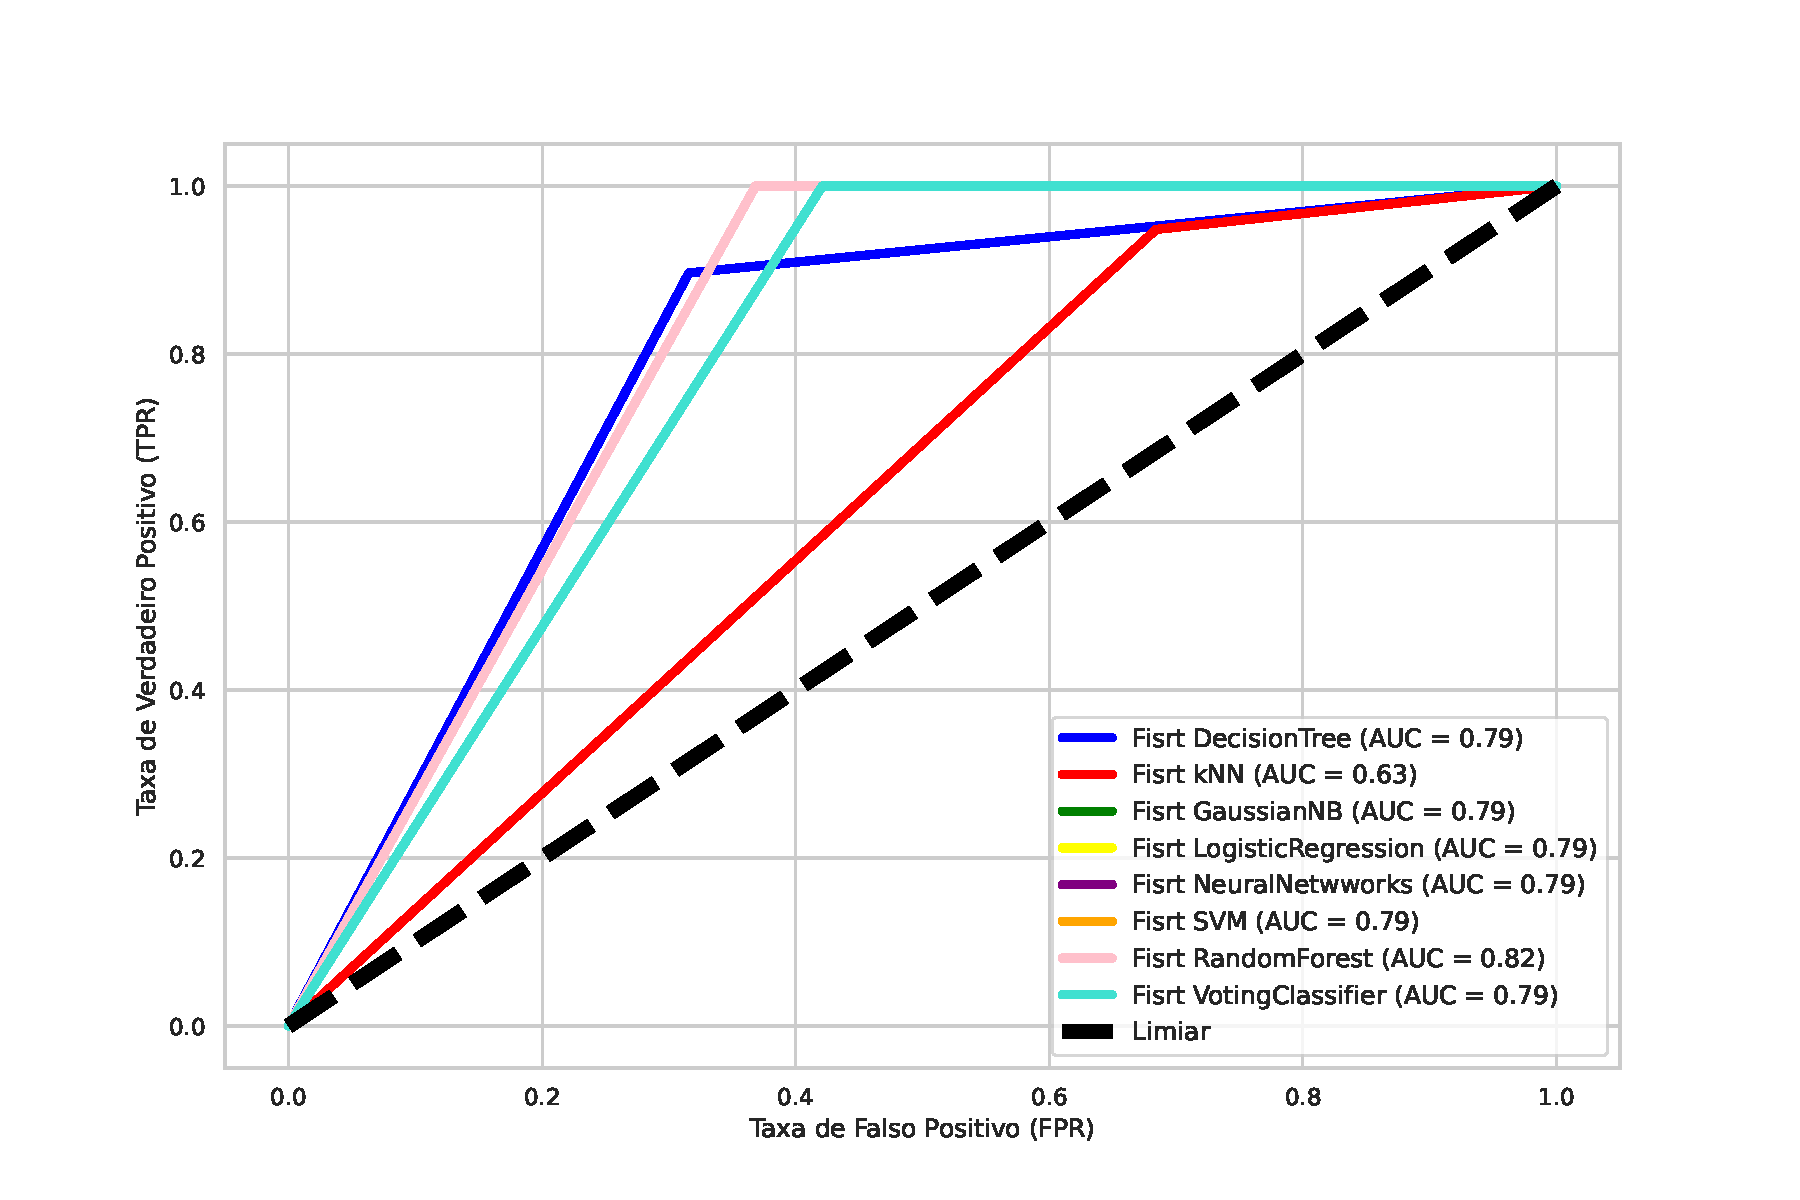
\includegraphics[scale=0.6]{Figures/CurvaROC_MI.pdf}
     \label{fig:7}
     Fonte: Elaborado pelo autor.
 \end{figure}

Tendo em mãos as informações de cada critério de avaliação, o modelo de classificação Florestas Aleatórias foi observado como o melhor dos \textit{Modelos Iniciais}, com uma acurácia de 90,91\%, tendo apenas 7 instâncias classificadas incorretamente. A Curva ROC obtida é bem satisfatória, tendo um AUC medido de 0,82.

\subsubsection{Modelos Finais}
Esta etapa destina-se à apresentação dos resultados do \textit{Modelos Finais} e avaliação dos mesmos. Para obtenção de tais resultados foi usado o Código (32), mostrado  a seguir.
\begin{center}
\textbf{Código 32:} Matriz de Confusão e Acurácia por Modelo Final.
\begin{minted}[linenos, fontsize=\footnotesize, bgcolor=bg]{python}
name_classifier = ['Last DecisionTree', 'Last kNN', 'Last LogisticRegression',
                   'Last NeuralNetwworks', 'Last SVM', 'Last RandomForest']
predict_classifier = [last_treeP, last_kNNP, last_lgP,
                      last_mlpP, last_svmP, last_randomforestP]

for i, j in zip(name_classifier, predict_classifier):
    # Métricas do classificador
    acuracy = accuracy_score(j, y_test) * 100
    # Printa as informações
    print(f'O classificador de {i}, obteve uma acurácia de {round(acuracy, 2)}%')

    # Matriz de confusão
    confusion_matrix = pd.DataFrame(cm(y_test, first_treeP),
                                    columns=['N (estimado)', 'Y (estimado)'],
                                    index=['N (original)', 'Y (original)'])
    print(confusion_matrix)
    print('--' * 50)
\end{minted}
\end{center}

Estão dispostas as informações da saída do Código (32) de forma tabelada, veja a Tabela (\ref{tab:5}) que contém a \textit{Matriz de Confusão} e \textit{Acurácia} de cada modelo.
\begin{table}[H]
    \centering
    \caption{Matriz de Confusão e Acurácia por Modelo Final.} 
    \begin{tabular}{ccc|c|c} \\ \hline
         \multicolumn{3}{c|}{Matriz de Confusão} & Modelo & Acurácia \\\hline
         & N (estimado) & Y (estimado) & \multirow{3}{*}{Árvore de Decisão} & \multirow{3}{*}{92,21\%} \\
         N (real) & 15 & 4 &  & \\
         Y (real) & 2 & 56 &  & \\ \hline
         & N (estimado) & Y (estimado) & \multirow{3}{*}{kNN} & \multirow{3}{*}{87,01\%}\\
         N (real) & 11 & 8 &  & \\
         Y (real) & 2 & 56 &  & \\ \hline
         & N (estimado) & Y (estimado) & \multirow{3}{*}{Regressão Logística} & \multirow{3}{*}{89,61\%}\\
         N (real) & 11 & 8 &  & \\
         Y (real) & 0 & 58 &  & \\  \hline
         & N (estimado) & Y (estimado) & \multirow{3}{*}{Redes Neurais} & \multirow{3}{*}{90,91\%}\\
         N (real) & 12 & 7 &  & \\
         Y (real) & 0 & 58 &  & \\ \hline
         & N (estimado) & Y (estimado) & \multirow{3}{*}{SVM} & \multirow{3}{*}{89,61\%}\\
         N (real) & 11 & 8 &  & \\
         Y (real) & 0 & 58 &  & \\ \hline
         & N (estimado) & Y (estimado) & \multirow{3}{*}{Florestas Aleatórias} & \multirow{3}{*}{90,91\%}\\
         N (real) & 12 & 7 &  & \\
         Y (real) & 0 & 58 &  & \\ \hline\hline
    \end{tabular} \\
    \label{tab:5}
    Fonte: Elaborado pelo autor.
\end{table}

A curva ROC de cada classificador da etapa de \textit{Modelos Iniciais}, encontrasse na Figura (\ref{fig:8}). Mas foi obtida com o o Código (33).
\begin{center}
\textbf{Código 33:} Curva ROC para os Modelos Iniciais.
\begin{minted}[linenos, fontsize=\footnotesize, bgcolor=bg]{python}
plt.figure(figsize=(12, 8), dpi=300)

colors = ['blue', 'red', 'green', 'yellow',
          'purple', 'orange']


# Plotar a curva ROC para cada modelo
for model_name, prediction, color in zip(name_classifier, predict_classifier, colors):
  fpr, tpr, _ = roc_curve(y_test, prediction)
  roc_auc = auc(fpr, tpr)

  sns.lineplot(x=fpr, y=tpr, label=f"{model_name} (AUC = {roc_auc:.2f})",
      linestyle="-", linewidth=4, color=color)

sns.lineplot(x=[0, 1], y=[0, 1],
    linestyle="--", label="Limiar",linewidth=7,color="black")

# Configurações do gráfico
plt.xlabel('Taxa de Falso Positivo (FPR)', fontsize=12)
plt.ylabel('Taxa de Verdadeiro Positivo (TPR)', fontsize=12)
plt.legend(prop={'size': 14}, loc='lower right')
plt.tight_layout()
plt.savefig('CurvaROC_MF.pdf', format='pdf', dpi=300, bbox_inches='tight')
plt.show()
\end{minted}
\end{center}

Veja a saída do Código (33), a Figura (\ref{fig:8}).
 \begin{figure}[H]
     \centering
     \caption{Curva ROC para os Modelos Finais.}
     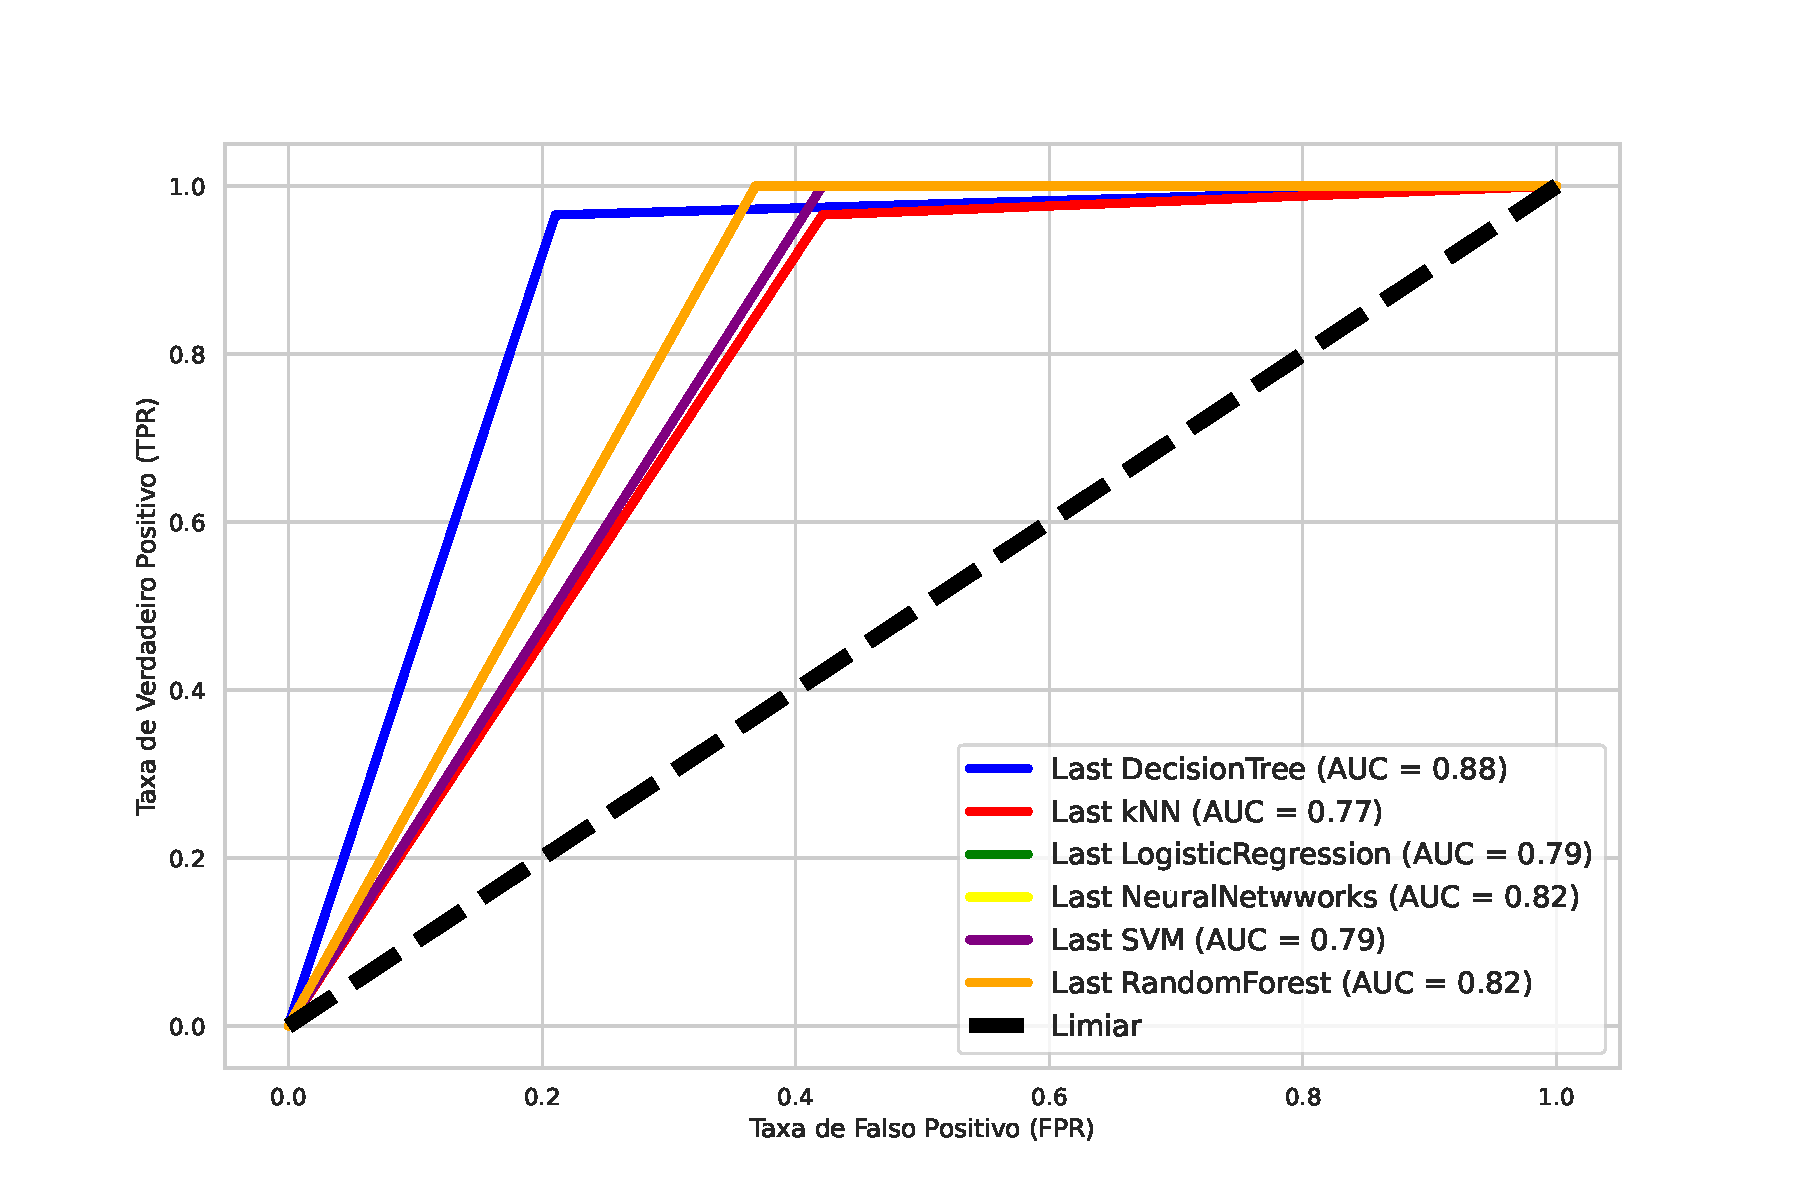
\includegraphics[scale=0.55]{Figures/CurvaROC_MF.pdf}
     \label{fig:8}
     Fonte: Elaborado pelo autor.
 \end{figure}
 
Dados o resultados obtidos, o classificador Árvore de Decisão foi identificado como o melhor dos \textit{Modelos Finais}, com uma acurácia de 92,21\%, e com apenas 6 instâncias classificadas incorretamente. A Curva ROC obtida é mostra uma boa capacidade de classificação do modelo, tendo um AUC de 0,88.


\subsubsection{Avaliação Geral dos Modelos}
Destinada a comparação entre os \textit{Modelos Iniciais} e \textit{Modelos Finais} à apresentação dos resultados de forma geral. Para obtenção de tais resultados foi usado o Código (32), mostrado  a seguir.
\begin{center}
\textbf{Código 32:} Matriz de Confusão e Acurácia de todos os Modelos.
\begin{minted}[linenos, fontsize=\footnotesize, bgcolor=bg]{python}
name_classifier = ['Fisrt DecisionTree', 'Fisrt kNN', 'Fisrt GaussianNB',
                   'Fisrt NeuralNetwworks', 'Fisrt SVM', 'Fisrt RandomForest',
                   'Fisrt VotingClassifier', 'Last DecisionTree', 'Last kNN',
                   'Last NeuralNetwworks', 'Last SVM', 'Last RandomForest',
                   'Last VotingClassifier']
predict_classifier = [first_treeP, first_kNNP, first_gnbP, first_mlpP,
                      first_svmP, first_randomforestP, first_votingP,
                      last_treeP, last_kNNP, last_mlpP, last_svmP, last_randomforestP]

for i, j in zip(name_classifier, predict_classifier):
    # Métricas do classificador
    acuracy = accuracy_score(y_test, j) * 100
    # Printa as informações
    print(f'O classificador de {i}, obteve uma acurácia de {round(acuracy, 2)}%')

    # Matriz de confusão
    confusion_matrix = pd.DataFrame(cm(y_test, first_treeP),
                                    columns=['N (estimado)', 'Y (estimado)'],
                                    index=['N (original)', 'Y (original)'])
    print(confusion_matrix)
    print('--' * 50)
\end{minted}
\end{center}

Estão dispostas as informações da saída do Código (32) de forma tabelada, veja a Tabela (\ref{tab:6}) que contém a \textit{Matriz de Confusão} e \textit{Acurácia} de cada modelo.
\begin{table}[H]
    \centering
    \caption{Matriz de Confusão e Acurácia de todos os Modelos.} 
    \begin{tabular}{ccc|c|c} \\ \hline
         \multicolumn{3}{c|}{Matriz de Confusão} & Modelo & Acurácia \\\hline
         & N (estimado) & Y (estimado) & \multirow{3}{*}{Árvore de Decisão$^1$} & \multirow{3}{*}{84,42\%} \\
         N (real) & 13 & 6 &  & \\
         Y (real) & 6 & 52 &  & \\ \hline
         & N (estimado) & Y (estimado) & \multirow{3}{*}{kNN$^1$} & \multirow{3}{*}{79,22\%}\\
         N (real) & 6 & 13 &  & \\
         Y (real) & 3 & 55 &  & \\ \hline
         & N (estimado) & Y (estimado) & \multirow{3}{*}{Naive Bayes} & \multirow{3}{*}{89,61\%}\\
         N (real) & 11 & 8 &  & \\
         Y (real) & 0 & 58 &  & \\ \hline
         & N (estimado) & Y (estimado) & \multirow{3}{*}{Regressão Logística$^1$} & \multirow{3}{*}{89,61\%}\\
         N (real) & 11 & 8 &  & \\
         Y (real) & 0 & 58 &  & \\  \hline
         & N (estimado) & Y (estimado) & \multirow{3}{*}{Redes Neurais$^1$} & \multirow{3}{*}{89,61\%}\\
         N (real) & 11 & 8 &  & \\
         Y (real) & 0 & 58 &  & \\ \hline
         & N (estimado) & Y (estimado) & \multirow{3}{*}{SVM$^1$} & \multirow{3}{*}{89,61\%}\\
         N (real) & 11 & 8 &  & \\
         Y (real) & 0 & 58 &  & \\ \hline
         & N (estimado) & Y (estimado) & \multirow{3}{*}{Florestas Aleatórias$^1$} & \multirow{3}{*}{90,91\%}\\
         N (real) & 12 & 7 &  & \\
         Y (real) & 0 & 58 &  & \\ \hline
         & N (estimado) & Y (estimado) & \multirow{3}{*}{Classificação por Votação} & \multirow{3}{*}{89,61\%}\\
         N (real) & 11 & 8 &  & \\
         Y (real) & 0 & 58 &  & \\ \hline
         & N (estimado) & Y (estimado) & \multirow{3}{*}{Árvore de Decisão$^2$} & \multirow{3}{*}{92,21\%} \\
         N (real) & 15 & 4 &  & \\
         Y (real) & 2 & 56 &  & \\ \hline
         & N (estimado) & Y (estimado) & \multirow{3}{*}{kNN$^2$} & \multirow{3}{*}{87,01\%}\\
         N (real) & 11 & 8 &  & \\
         Y (real) & 2 & 56 &  & \\ \hline
         & N (estimado) & Y (estimado) & \multirow{3}{*}{Regressão Logística$^2$} & \multirow{3}{*}{89,61\%}\\
         N (real) & 11 & 8 &  & \\
         Y (real) & 0 & 58 &  & \\  \hline
         & N (estimado) & Y (estimado) & \multirow{3}{*}{Redes Neurais$^2$} & \multirow{3}{*}{90,91\%}\\
         N (real) & 12 & 7 &  & \\
         Y (real) & 0 & 58 &  & \\ \hline
         & N (estimado) & Y (estimado) & \multirow{3}{*}{SVM$^2$} & \multirow{3}{*}{89,61\%}\\
         N (real) & 11 & 8 &  & \\
         Y (real) & 0 & 58 &  & \\ \hline
         & N (estimado) & Y (estimado) & \multirow{3}{*}{Florestas Aleatórias$^2$} & \multirow{3}{*}{90,91\%}\\
         N (real) & 12 & 7 &  & \\
         Y (real) & 0 & 58 &  & \\ \hline\hline
    \end{tabular} \\
    \label{tab:6}
    Fonte: Elaborado pelo autor.
\end{table}

 A curva ROC de cada classificador, encontrasse na Figura (\ref{fig:9}). Mas foi obtida com o o Código (34).
\begin{center}
\textbf{Código 34:} Curva ROC para todos os Modelos.
\begin{minted}[linenos, fontsize=\footnotesize, bgcolor=bg]{python}
plt.figure(figsize=(12, 8), dpi=300)

colors = ['blue', 'red', 'green', 'yellow',
          'purple', 'orange', 'pink', 'turquoise',
          'brown', 'gray', 'lightblue',
          'lightgreen', 'violet', 'gold']

# Plotar a curva ROC para cada modelo
for model_name, prediction, color in zip(name_classifier, predict_classifier, colors):
  fpr, tpr, _ = roc_curve(y_test, prediction)
  roc_auc = auc(fpr, tpr)

  sns.lineplot(x=fpr, y=tpr, label=f"{model_name} (AUC = {roc_auc:.2f})",
               linestyle="-", linewidth=2.5, color=color)

sns.lineplot(x=[0, 1], y=[0, 1],
             linestyle="--", label="Limiar",linewidth=7,color="black")

# Configurações do gráfico
plt.xlabel('Taxa de Falso Positivo (FPR)', fontsize=12)
plt.ylabel('Taxa de Verdadeiro Positivo (TPR)', fontsize=12)
plt.legend(prop={'size': 12}, loc='lower right')
plt.tight_layout()
plt.savefig('CurvaROC_AG.pdf', format='pdf', dpi=300, bbox_inches='tight')
plt.show()
\end{minted}
\end{center}

Veja a saída do Código (34), a Figura (\ref{fig:9}).
 \begin{figure}[H]
     \centering
     \caption{Curva ROC para os todos os Modelos.}
     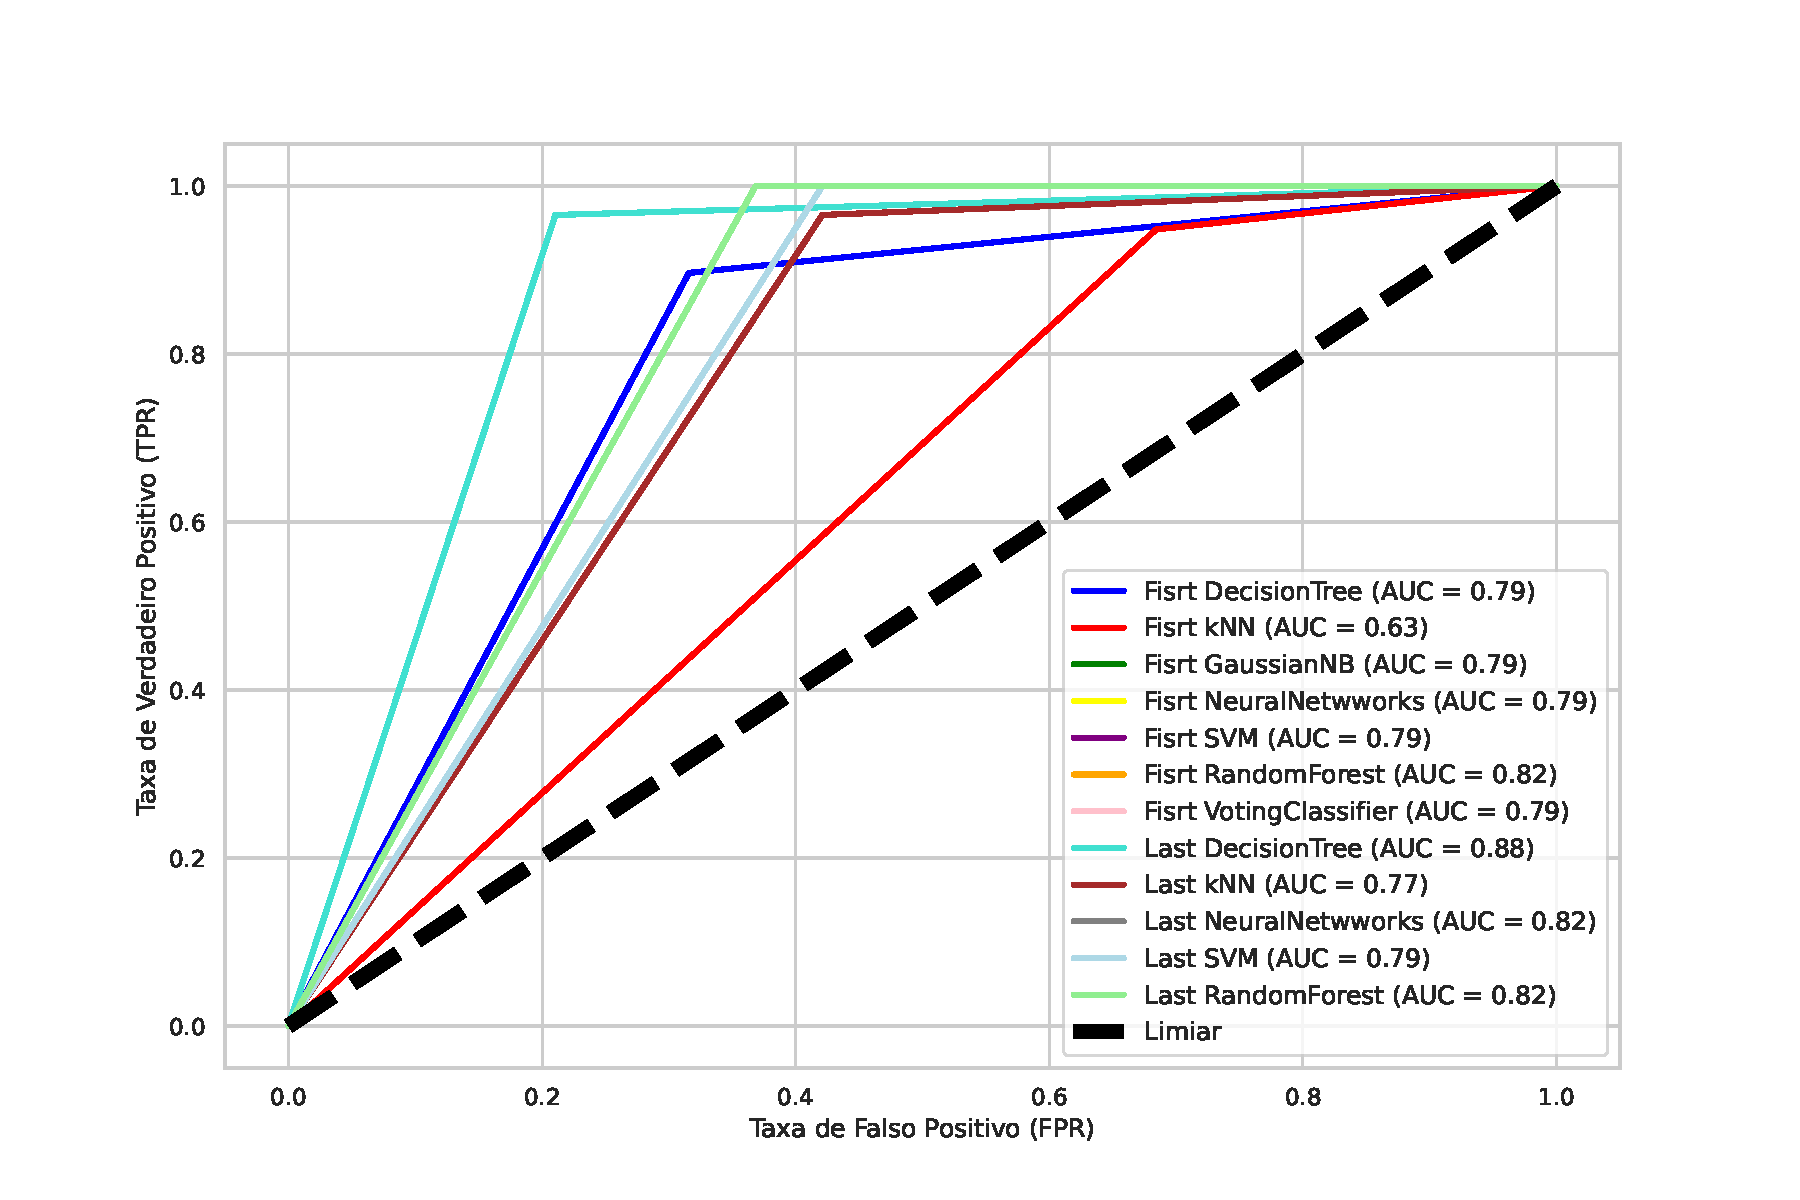
\includegraphics[scale=0.55]{Figures/CurvaROC_AG.pdf}
     \label{fig:9}
     Fonte: Elaborado pelo autor.
 \end{figure}

Com base nos resultados encontrados, a Árvore de Decisão se destacou como o modelo mais eficaz, alcançando uma taxa de acurácia de 92,21\% e classificando incorretamente apenas 6 instâncias. Além disso, a análise da Curva ROC revelou um AUC de 0,88, o que demonstra um desempenho satisfatório e uma boa capacidade preditiva do modelo.

\section{Conclusão}
O modelo de \textit{Árvore de Decisão}, de hiperparâmetros que constam na Tabela (\ref{tab:3}), se destaca na previsão do status de empréstimo, alcançando uma acurácia de 92,21\%, com apenas 6 erros em 77 instâncias avaliadas. A análise da matriz de confusão demonstra uma precisão alta, superando outros modelos como \textit{Redes Neurais}, \textit{Regressão Logística}, \textit{Florestas Aleatórias}, \textit{SVM} entre outros. Usando a semente de número 16.

A Curva ROC do modelo exibe uma AUC de 0,88, validando sua capacidade de diferenciar entre classes positivas (empréstimo aprovado) e negativas (empréstimo negado), evidenciando sua robustez e capacidade de generalização para novos dados.

Esses resultados afirmam o modelo de \textit{Árvore de Decisão} como a melhor escolha para prever o status de empréstimo, destacando sua confiabilidade, robustez e capacidade de generalização. Essa ferramenta é crucial para instituições financeiras em busca de otimização de processos de análise de crédito.

Sugere-se a complementação da análise com métricas adicionais, como F1-score e tempo de treinamento, entre outras, além da comparação mais aprofundada com outros modelos de classificação. Explorar a interpretabilidade que o modelo de \textit{Árvore de Decisão} pode proporcionar, como insights sobre as características que influenciam as decisões de aprovação ou negação de empréstimo por exemplo. Outros sugestões seriam sobre o tamanho dos conjuntos de treino e teste, ou até mesmo sobre a definição de outra semente, podendo encontrar uma semente que maximize as métricas usadas para avaliar, como acurácia. Pode se tornar decisivo também, encontrar outras variáveis e atributos que sejam fortemente correlacionados com a coluna alvo (\textit{Loan\_Status}) e que auxiliem no processo de classificação.

\newpage
%Sets the bibliography style to UNSRT and imports the 
%bibliography file "sample.bib".
\bibliographystyle{unsrt}
\bibliography{references}

\end{document}
